% ===========================================================================
% Cassini ISS F Ring Mosaics User Guide
% Converted to LaTeX from users-guide-draft-phase2-6.docx
%
% Build:  make            (or: pdflatex main.tex, three times)
% See README.md for notes on font substitutions and the pending
% bibliography (Zotero -> BibTeX) pass.
% ===========================================================================
\documentclass[12pt,letterpaper]{article}

% ---------------------------------------------------------------------------
% Preamble for the Cassini ISS F Ring Mosaics User Guide
% Converted from users-guide-draft-phase2-6.docx
% ---------------------------------------------------------------------------

\usepackage[utf8]{inputenc}
\usepackage[T1]{fontenc}
\usepackage{textcomp}

% Base fonts: Times body (Word: Times New Roman/Minion), Helvetica for
% headings (Word: Calibri), Courier for code (Word: Cascadia Code).
\usepackage{mathptmx}
\usepackage[scaled=0.92]{helvet}
\usepackage{courier}

% Page geometry matches the Word original (US Letter,
% margins: left/right/top 0.75 in, bottom 1.25 in).
\usepackage[letterpaper,left=0.75in,right=0.75in,top=0.75in,bottom=1.25in,
            footskip=0.5in]{geometry}

\usepackage{graphicx}
\usepackage{longtable}
\usepackage{array}
\usepackage{amsmath}
\usepackage{amssymb}
\usepackage{fancyvrb}
\usepackage{fvextra}     % adds automatic line breaking to verbatim blocks
\usepackage{float}
\usepackage{enumitem}
\usepackage{titlesec}
\usepackage{caption}
\usepackage{fancyhdr}
\usepackage{pmboxdraw}      % box-drawing characters in directory listings
\usepackage{newunicodechar}
\usepackage{lscape}         % Section 7 is landscape, as in the Word original
\usepackage{lastpage}

% Rotate the physical PDF pages of landscape sections (equivalent to
% pdflscape, but implemented directly for maximum portability).
\ifdefined\pdfpageattr
  \newenvironment{rotatedlandscape}
    {\clearpage\global\pdfpageattr{/Rotate 90}\begin{landscape}}
    {\end{landscape}\clearpage\global\pdfpageattr{}}
\else
  \newenvironment{rotatedlandscape}
    {\begin{landscape}}{\end{landscape}}
\fi

% --- characters used in the Word source ------------------------------------
\newunicodechar{°}{\textdegree}
\newunicodechar{−}{\ensuremath{-}}
\newunicodechar{×}{\ensuremath{\times}}
\newunicodechar{Δ}{\ensuremath{\Delta}}
\newunicodechar{ϖ}{\ensuremath{\varpi}}
\newunicodechar{Ω}{\ensuremath{\Omega}}
\newunicodechar{λ}{\ensuremath{\lambda}}
\newunicodechar{θ}{\ensuremath{\theta}}
\newunicodechar{≈}{\ensuremath{\approx}}

% --- paragraph layout: 0.25 in first-line indent, no inter-paragraph skip,
% as in the Word original
\setlength{\parindent}{0.25in}
\setlength{\parskip}{0pt}
\emergencystretch=1em

% --- headings: numbered to 4 levels (Word Heading 1-4); TOC to 3 levels ----
\setcounter{secnumdepth}{4}
\setcounter{tocdepth}{3}

% Sizes/weights follow the Word styles:
%   Heading 1: 16 pt bold;  Heading 2: 13 pt bold;
%   Heading 3 and 4: 12 pt bold italic
\titleformat{\section}
  {\headingfont\fontsize{16pt}{19pt}\selectfont}{\thesection}{0.6em}{}
\titlespacing*{\section}{0pt}{6pt}{12pt}
\titleformat{\subsection}
  {\headingfont\fontsize{13pt}{16pt}\selectfont}{\thesubsection}{0.6em}{}
\titlespacing*{\subsection}{0pt}{12pt}{6pt}
\titleformat{\subsubsection}
  {\headingfont\itshape\fontsize{12pt}{14pt}\selectfont}{\thesubsubsection}{0.6em}{}
\titlespacing*{\subsubsection}{0pt}{12pt}{6pt}
\titleformat{\paragraph}[hang]
  {\headingfont\itshape\fontsize{12pt}{14pt}\selectfont}{\theparagraph}{0.6em}{}
\titlespacing*{\paragraph}{0pt}{6pt}{6pt}

% --- captions: "Figure N: ..." in italics, as in the Word Caption style ----
\captionsetup{labelsep=colon,font={it},skip=6pt}

% --- lists: compact spacing similar to Word --------------------------------
\setlist{itemsep=2pt,topsep=4pt,parsep=0pt}

% --- tables ----------------------------------------------------------------
\setlength{\LTpre}{8pt}
\setlength{\LTpost}{8pt}
\renewcommand{\arraystretch}{1.15}

% --- footer: "Page N of M" centered, as in the Word original ---------------
\pagestyle{fancy}
\fancyhf{}
\fancyfoot[C]{\small Page \thepage\ of \pageref{LastPage}}
\renewcommand{\headrulewidth}{0pt}
\fancypagestyle{plain}{\fancyhf{}%
  \fancyfoot[C]{\small Page \thepage\ of \pageref{LastPage}}}

% --- hyperlinks ------------------------------------------------------------
% hyperref last; URLs blue as in Word, internal cross-references black
\usepackage[colorlinks=true,urlcolor=blue,linkcolor=black,citecolor=black,
            pdftitle={Cassini ISS F Ring Mosaics User Guide},
            pdfauthor={Robert S. French}]{hyperref}

% allow URLs to break more freely and stretch slightly
\Urlmuskip=0mu plus 2mu
% \allowbreak appears in some heading code tokens; ignore it in PDF bookmarks
\pdfstringdefDisableCommands{\let\allowbreak\relax}

% long URLs (e.g. in the References section) may break after any character
\expandafter\def\expandafter\UrlBreaks\expandafter{\UrlBreaks%
  \do\a\do\b\do\c\do\d\do\e\do\f\do\g\do\h\do\i\do\j\do\k\do\l\do\m%
  \do\n\do\o\do\p\do\q\do\r\do\s\do\t\do\u\do\v\do\w\do\x\do\y\do\z%
  \do\0\do\1\do\2\do\3\do\4\do\5\do\6\do\7\do\8\do\9\do\-\do\_}

% ---------------------------------------------------------------------------
% Font macros for the F Ring User's Guide
%
% The Word original uses several distinctive fonts that are not generally
% available to LaTeX.  Each is wrapped in a macro here so the font choice can
% be changed in ONE place.  Current substitutions:
%
%   Word font           Used for                          LaTeX substitute
%   ------------------  --------------------------------  -----------------------
%   Times New Roman     body text, title                  Times (mathptmx)
%   Calibri (bold)      headings                          Helvetica (phv)
%   Cascadia Code       file names, program constants,    Courier (pcr)
%                       code blocks, directory listings
%   Courier New         "Literal" style (rarely used)     Courier (pcr)
%   Lucida Sans         (label listings in older drafts;  Helvetica (phv)
%                       retained for completeness)
%
% If you compile on a full TeX system you may prefer, e.g.:
%   \renewcommand{\codefontfamily}{\fontfamily{zi4}\selectfont}   % Inconsolata
% or with LuaLaTeX/XeLaTeX + fontspec, set these to the real fonts.
% ---------------------------------------------------------------------------

% --- inline font for file names / program constants (Word: Cascadia Code)
\newcommand{\codefontfamily}{\fontfamily{pcr}\selectfont}
\newcommand{\code}[1]{{\codefontfamily #1}}

% --- inline font for the Word "Literal" character style (Word: Courier New)
\newcommand{\literalfontfamily}{\fontfamily{pcr}\selectfont}
\newcommand{\literal}[1]{{\literalfontfamily #1}}

% --- inline font for XML label excerpts in older drafts (Word: Lucida Sans)
\newcommand{\labelxmlfontfamily}{\fontfamily{phv}\selectfont}
\newcommand{\labelxml}[1]{{\labelxmlfontfamily #1}}

% --- heading font (Word: Calibri bold)
\newcommand{\headingfont}{\sffamily\bfseries}

% --- title font (Word: Times New Roman 18 pt bold)
\newcommand{\usgtitlefont}{\rmfamily\bfseries\fontsize{18pt}{22pt}\selectfont}

% --- Zotero citation placeholder.
% The Word document manages citations with Zotero.  Until the bibliography is
% converted to BibTeX (second pass), \zcite simply prints the plain citation
% text captured from the Word field.  The full CSL JSON data for every
% citation was extracted to citations/zotero-citations.json.
\newcommand{\zcite}[1]{#1}

% --- verbatim environments for code blocks --------------------------------
% CodeBlock    : Word "Code" style paragraphs (Cascadia Code)
% LiteralBlock : Word "Literal" style paragraphs (Courier New)
% LabelBlock   : XML label listings (Lucida Sans in older drafts)
% A [fontsize=...] option is emitted by the converter where the Word source
% used a smaller point size (e.g. the long XML label listings).
% breaklines wraps lines too long for the page, as Word does; the
% continuation line is indented and unmarked (set breaksymbolleft to change).
\DefineVerbatimEnvironment{CodeBlock}{Verbatim}%
  {fontsize=\small,formatcom=\codefontfamily,xleftmargin=1.5em,
   breaklines=true,breakanywhere=true,breaksymbolleft={},breakindent=2em}
\DefineVerbatimEnvironment{LiteralBlock}{Verbatim}%
  {fontsize=\small,formatcom=\literalfontfamily,xleftmargin=1.5em,
   breaklines=true,breakanywhere=true,breaksymbolleft={},breakindent=2em}
\DefineVerbatimEnvironment{LabelBlock}{Verbatim}%
  {fontsize=\small,formatcom=\labelxmlfontfamily,xleftmargin=1.5em,
   breaklines=true,breakanywhere=true,breaksymbolleft={},breakindent=2em}


\begin{document}

% --- title block (Word title page, which flows into the TOC) ---------------
\begin{center}
{\usgtitlefont Cassini ISS F Ring Mosaics User Guide\par}
\end{center}

\begin{center}
V1.0
\end{center}

\begin{center}
Robert S. French (\href{mailto:rfrench@seti.org}{rfrench@seti.org})
\end{center}

\begin{center}
Carl Sagan Center, SETI Institute, Mountain View, CA 94043
\end{center}

\begin{center}
DOI: 10.17189/ajhh-aj88
\end{center}

\vspace{2em}

\begin{center}
\begin{minipage}{0.88\linewidth}
\small

\noindent\textbf{Citing this bundle.} French, R. S., \& Hedman, M. M. (2026).
\textit{F Ring Mosaics and Reprojected Images Created from Calibrated Cassini ISS
Images, and Associated Metadata} (Version 1.0) [Data set]. NASA Planetary Data System.
\url{https://doi.org/10.17189/3tfh-th07}

\vspace{0.75em}

\noindent\textbf{Citing this User Guide.} French, R. S. (2026).
\textit{Cassini ISS F Ring Mosaics User Guide} (Version 1.0). NASA Planetary Data
System. \url{https://doi.org/10.17189/ajhh-aj88}

\vspace{0.75em}

\noindent\textbf{Versions and errata.} This is Version 1.0 of the bundle and of this
\textit{User Guide}. The bundle version is recorded in the \code{version\_\allowbreak{}id}
of every label, and each label carries a \code{Modification\_\allowbreak{}History}
describing what changed in each version. Corrections made after release are issued as a
new version of the bundle, with a new \code{Modification\_\allowbreak{}Detail} entry
recording the change and a reissue of this \textit{User Guide} at the matching version.
Errata identified between releases are posted with the bundle at the PDS Ring-Moon Systems
Node (\url{https://pds-rings.seti.org/}). Please report suspected errors to
\href{mailto:rfrench@seti.org}{rfrench@seti.org}.

\end{minipage}
\end{center}

%% Table of contents (Word TOC replaced by LaTeX)


\tableofcontents
\clearpage

% Section 1: Introduction

\section{Introduction}
\label{sec:introduction}

Saturn’s F ring is one of the most dynamic and scientifically intriguing features in the solar system. Discovered in 1979 by the Pioneer 11 spacecraft \zcite{(Gehrels et al. 1980)}, the F ring is a narrow, complex, and ever-changing structure located just outside Saturn’s main ring system. Its unique morphology, characterized by multiple strands, clumps, and transient features, along with the influence of neighboring moons Prometheus and Pandora, has made it a focal point for studies of planetary ring dynamics, satellite-ring interactions, and the processes governing the evolution of ring systems.

Before 2004, quality images of the F ring were limited to a handful produced by the Voyager 1 and 2 spacecraft during their short fly-bys in 1980 and 1981. This all changed with the arrival of the Cassini Orbiter at Saturn on June 30, 2004. During its subsequent 13 years at Saturn, Cassini used its Imaging Science Subsystem (ISS) \zcite{(Knowles 2018; Porco et al. 2004)} to observe the F ring more than 100,000 times, providing a treasure trove of data that is unlikely to be surpassed for generations.

This \textit{User Guide} provides a detailed description of the organization and contents of the Cassini ISS F Ring Mosaics bundle archived at NASA’s Planetary Data System Ring-Moon Systems Node under NASA CDAP grant 80NSSC21K0527: “The recent history of Saturn's dusty rings”. The purpose of this archive is to provide a carefully curated and documented set of high-quality images of the F ring taken by the ISS Narrow Angle Camera (NAC) and Wide Angle Camera (WAC) \zcite{(Porco et al. 2004)} using clear filters. Special emphasis is placed on “FMOVIEs”, sequences of dozens to hundreds of images taken in rapid succession at a single inertial longitude while the F ring orbited through the field of view. Such movies provide a detailed picture of the F ring material at various corotating longitudes as it passes through some true anomaly in the F ring’s eccentric orbit.

All included images were calibrated in units of I/F using CISSCAL 4.0 \zcite{(Knowles 2018)} and then reprojected onto a grid with radius relative to the F ring core on the vertical axis and corotating longitude on the horizontal axis (see Section \ref{sec:reprojection}). Multiple images were stitched together to form more complete mosaics, and the mosaics were then analyzed to remove any background gradient.

The archive includes reprojected images, mosaics, and mosaics that have been adjusted by subtracting a background model, organized by Cassini “observation name” (see Section \ref{sec:image-selection}). Each reprojected image and mosaic is supplemented by a table containing metadata such as resolution, phase angle, and emission angle for each valid corotating longitude. Reprojected images have an additional file describing the spacecraft pointing used to perform the reprojection. Mosaics have an additional file listing the reprojected images that were used to create the mosaic. A series of browse images in various sizes is provided for each reprojected image and mosaic as well. In total 20,303 reprojected images are provided along with 305 associated mosaics.

Finally, three global index files are provided covering the complete set of reprojected images, mosaics, and background-subtracted mosaics. These index files summarize metadata such as time, corotating longitude coverage, lighting and viewing geometry, and orbit details for each data product, making it easy to search for and analyze the data products \textit{en masse}.

First time users are encouraged to read or skim this entire \textit{User Guide} at least once (and possibly twice) before making use of the archived results.

\clearpage
% Section 2: Quick start

\section{Quick start}
\label{sec:quick-start}

The data set described here is archived using the PDS4 standard. While deep knowledge of PDS4 is not required to make use of the data, some familiarity is useful. Specifications, tools, and training are available from the main PDS website at \href{https://pds.nasa.gov}{https://pds.nasa.gov}.\footnote{Refer to the documents in Section~\ref{sec:pds4-standards-and-documentation} for further information on the PDS4 concepts of \textit{bundle}, \textit{collection}, and \textit{data product}.}

This data is archived as a single PDS4 \textit{bundle}, which consists of multiple \textit{collections}. Each collection represents one particular type of data (reprojected images, mosaics, browse images, etc.). Within a collection, individual data products are described by a \textit{label} (suffix \code{.\allowbreak{}lblx}), which contains substantial information about the data product, including details of any associated binary image (\code{.\allowbreak{}img}), graphical image (\code{.\allowbreak{}png}), metadata table (\code{.\allowbreak{}tab}), or supplemental (\code{.\allowbreak{}txt}) files.

Data product files are best read by first processing the associated label file, extracting the needed metadata about the data product, and then using the information in the label to identify the file(s) to read and the details of their format. Special software is available in a variety of programming languages for processing labels and reading the associated data products (Section~\ref{sec:reading-labels-and-data-product-files}).

Below is a summary of the collections related to reprojected images and the files contained within each.

\begingroup\small
\begin{longtable}{|>{\raggedright\arraybackslash}p{0.186\linewidth}|>{\raggedright\arraybackslash}p{0.405\linewidth}|>{\raggedright\arraybackslash}p{0.329\linewidth}|}
\hline
Collection & Filename(s) & Description \\
\hline
\code{browse\_\allowbreak{}reproj\_\allowbreak{}img} (Section~\ref{sec:browse-reproj-img}) & \code{IMGID\_\allowbreak{}browse\_\allowbreak{}reproj\_\allowbreak{}img.\allowbreak{}lblx} & PDS4 label describing the four types of browse images for reprojected image data. \\
\hline
 & \code{IMGID\_\allowbreak{}browse\_\allowbreak{}reproj\_\allowbreak{}img\_\allowbreak{}full.\allowbreak{}png}\newline \code{IMGID\_\allowbreak{}browse\_\allowbreak{}reproj\_\allowbreak{}img\_\allowbreak{}med.\allowbreak{}png} \newline \code{IMGID\_\allowbreak{}browse\_\allowbreak{}reproj\_\allowbreak{}img\_\allowbreak{}small.\allowbreak{}png} \newline \code{IMGID\_\allowbreak{}browse\_\allowbreak{}reproj\_\allowbreak{}img\_\allowbreak{}thumb.\allowbreak{}png} & Human-viewable versions of reprojected images in four sizes in standard PNG format. Images are contrast-stretched and not calibrated for scientific use. \\
\hline
\code{data\_\allowbreak{}reproj\_\allowbreak{}img} (Section~\ref{sec:data-reproj-img}) & \code{IMGID\_\allowbreak{}reproj\_\allowbreak{}img.\allowbreak{}lblx} & PDS4 label describing the reprojected image and the three associated data files. \\
\hline
 & \code{IMGID\_\allowbreak{}reproj\_\allowbreak{}img.\allowbreak{}img} & Binary file containing a 401×\textit{N} array of 32-bit floating-point values calibrated as I/F: 401 rows of radius in increments of 5 km, by \textit{N} columns of corotating longitude in 0.02° increments. The longitudes are restricted to the range containing valid data. \\
\hline
 & \code{IMGID\_\allowbreak{}reproj\_\allowbreak{}img\_\allowbreak{}metadata\_\allowbreak{}params.\allowbreak{}tab} & Fixed-width comma-delimited table containing metadata for each valid corotating longitude in the \code{reproj\_\allowbreak{}img}. \\
\hline
 & \code{IMGID\_\allowbreak{}reproj\_\allowbreak{}img\_\allowbreak{}suppl.\allowbreak{}txt} & Text file containing a description of the navigation results for the original Cassini ISS image and the resulting SPICE C matrix. \\
\hline
\end{longtable}
\endgroup

Below is a summary of the collections related to mosaics (and background-subtracted mosaics) and the files contained within each.

\begingroup\small
\begin{longtable}{|>{\raggedright\arraybackslash}p{0.222\linewidth}|>{\raggedright\arraybackslash}p{0.444\linewidth}|>{\raggedright\arraybackslash}p{0.254\linewidth}|}
\hline
Collection & Filename(s) & Description \\
\hline
\code{browse\_\allowbreak{}mosaic} [original]\newline \code{browse\_\allowbreak{}mosaic\_\allowbreak{}bkg\_\allowbreak{}sub}\newline [background gradient removed] (Section~\ref{sec:browse-mosaic-and-browse-mosaic-bkg-sub}) & \code{OBSID\_\allowbreak{}browse\_\allowbreak{}mosaic[\_\allowbreak{}bkg\_\allowbreak{}sub].\allowbreak{}lblx} & PDS4 label describing the four types of browse images for mosaic data. \\
\hline
 & \code{OBSID\_\allowbreak{}browse\_\allowbreak{}mosaic[\_\allowbreak{}bkg\_\allowbreak{}sub]\_\allowbreak{}full.\allowbreak{}png}\newline \code{OBSID\_\allowbreak{}browse\_\allowbreak{}mosaic[\_\allowbreak{}bkg\_\allowbreak{}sub]\_\allowbreak{}med.\allowbreak{}png} \newline \code{OBSID\_\allowbreak{}browse\_\allowbreak{}mosaic[\_\allowbreak{}bkg\_\allowbreak{}sub]\_\allowbreak{}small.\allowbreak{}png} \newline \code{OBSID\_\allowbreak{}browse\_\allowbreak{}mosaic[\_\allowbreak{}bkg\_\allowbreak{}sub]\_\allowbreak{}thumb.\allowbreak{}png} & Human-viewable versions of mosaics in four sizes in standard PNG format. Images are contrast-stretched and not calibrated for scientific use. \\
\hline
\code{data\_\allowbreak{}mosaic} [original]\newline \code{data\_\allowbreak{}mosaic\_\allowbreak{}bkg\_\allowbreak{}sub}\newline [background gradient removed] (Section~\ref{sec:data-mosaic-and-data-mosaic-bkg-sub}) & \code{OBSID\_\allowbreak{}mosaic[\_\allowbreak{}bkg\_\allowbreak{}sub].\allowbreak{}lblx} & PDS4 label describing the mosaic and the three associated data files. \\
\hline
 & \code{OBSID\_\allowbreak{}mosaic[\_\allowbreak{}bkg\_\allowbreak{}sub].\allowbreak{}img} & Binary file containing a 401×18,000 array of 32-bit floating-point values calibrated as I/F: 401 rows of radius in increments of 5 km, by 18,000 columns of corotating longitude in 0.02° increments. \\
\hline
 & \code{OBSID\_\allowbreak{}mosaic[\_\allowbreak{}bkg\_\allowbreak{}sub]\_\allowbreak{}metadata\_\allowbreak{}params.\allowbreak{}tab} & Fixed-width comma-delimited table containing metadata for each valid corotating longitude in the mosaic. \\
\hline
 & \code{OBSID\_\allowbreak{}mosaic[\_\allowbreak{}bkg\_\allowbreak{}sub]\_\allowbreak{}metadata\_\allowbreak{}src\_\allowbreak{}imgs.\allowbreak{}tab} & Fixed-width comma-delimited table containing a map of image numbers from the \code{metadata\_\allowbreak{}params} table to the associated reprojected image LIDVID. \\
\hline
\end{longtable}
\endgroup

Other collections are provided in the bundle, including a document collection containing this \textit{User Guide} and a miscellaneous collection containing global index files. All collections and support files are described in the sections below.

The remainder of this \textit{User Guide} provides detailed guidance on the use of the bundle:

\begin{itemize}
\item Section~\ref{sec:image-selection-and-processing} describes the selection and processing of Cassini ISS images and the creation of the mosaics, including the steps:
\begin{itemize}
\item Image selection (Section~\ref{sec:image-selection})
\item Image calibration (Section~\ref{sec:calibration})
\item Image navigation (pointing correction) (Section~\ref{sec:navigation})
\item Image reprojection (Section~\ref{sec:reprojection})
\item Mosaic creation (Section~\ref{sec:mosaic-creation})
\item Mosaic background gradient modeling and subtraction (Section~\ref{sec:background-modeling})
\end{itemize}
\item Section~\ref{sec:bundle-organization-and-directory-structure} describes the bundle organization and directory structure, including the details of all files included
\item Section~\ref{sec:reading-labels-and-data-product-files} discusses techniques for reading label and data product files
\item Section~\ref{sec:external-references-and-further-reading} contains useful external references
\item Section~\ref{sec:metadata-and-global-index-file-fields} provides an itemized list of all metadata fields and their meaning
\end{itemize}

\clearpage
% Section 3: Image selection and processing

\section{Image selection and processing}
\label{sec:image-selection-and-processing}


\subsection{Image selection}
\label{sec:image-selection}

Cassini observations were organized into observing campaigns. Each campaign was given a unique identifier (the observation name), which has the general format:

\begin{CodeBlock}
[INST]_[REV][TI]_[UNIQUENAME]_[PINST]
\end{CodeBlock}

where for the observations included in this bundle:

\begin{itemize}
\item INST is the abbreviation for the instrument being commanded (usually “ISS”)
\item REV is the rev (orbit) identifier, starting with 000 at Saturn orbit insertion and ending with 293 at the end of the mission. A few early revs are lettered instead of numbered; this bundle contains rev \code{00A}. Software that splits an observation name should treat REV as a fixed field of three characters and not assume it is an integer
\item TI is a 2-character target identifier: RA (A ring), RB (B ring), RF (F ring), RI (general rings), ST (star)
\item UNIQUENAME is a unique descriptor chosen by the observation creator, often containing acronyms such as “LP” for low phase, “HR” for high resolution, and “MOV” for movie. Some of the more common names:
\begin{itemize}
\item APOMOS* – Images taken at Cassini apoapse, often used to make large mosaics
\item AZSCN* – Azimuthal scan around the rings
\item *OCC – Stellar occultation
\item COMPLIT* – Radial composition scan on the lit side of the rings
\item EGAPMOVMP – Encke gap movie, medium phase
\item FMONITOR – F ring monitor; often an ISS rider on CIRS scans of the A and B rings
\item FMOVIE – Stared at a fixed inertial longitude to image F ring material passing through the field of view
\item FMOVIEEQX – F ring movie at Saturn equinox
\item FRSTRCHAN – Prometheus and F ring streamer-channel movie; tracks Prometheus and follows a small section of the F ring around one complete orbit
\item HIRESAFRG – High-resolution A ring outer edge
\item HIRESFRNG – High-resolution F ring
\item LATPHASE – Latitude and phase angle; wide range of sub-spacecraft latitude and solar phase angle
\item PROPRETRG – Re-targeting known “propeller” moons to track their orbits
\item SPK*, SPOKEMOV* – Spoke observation; stared at a ring ansa at regular intervals to watch B ring spokes move through the field of view
\item SUBM*, TDIFS*, TMAP* – Thermal observations by the Composite Infrared Spectrometer (CIRS); ISS rider
\item UR* – Ultraviolet Imaging Spectrograph (UVIS) ring stellar occultation; ISS rider
\end{itemize}
\item PINST indicates the name of the prime instrument if other than the ISS \zcite{(Knowles 2018)}. If PINST is not “PRIME”, then the ISS images were a ride-along on observations designed for the other instrument.
\end{itemize}
The complete set of $\sim$100,000 images containing the F ring was manually inspected for high-quality images.

In general, an image was included in our data set if:

\begin{enumerate}
\item It was a member of a series of images taken at different corotating longitudes that could be stitched together into a mosaic;
\item It was taken with the “clear” filters;
\item It was not corrupted or partially downloaded; and
\item Its best radial resolution at the F ring was no coarser than $\sim$80 km/pixel.
\end{enumerate}
However, due to the variation in image attributes and quality, the final determination of which images to include was necessarily subjective. For example:

\begin{itemize}
\item Some images were included that do not meet requirement \#1. If a single WAC image contained enough of the F ring to subjectively make a good mosaic by itself, it was included. Also, some image sequences were included where the camera followed a single corotating longitude as it traversed different inertial longitudes.
\item Some images were included that do not meet requirement \#4. These included the 42 “SPOKEMOV” mosaics taken at relatively low resolution by the WAC. While the reprojected images for these sequences are not of very high quality, the resulting mosaics are nevertheless sufficient for research, such as photometry, that does not require high-resolution analysis.
\end{itemize}
In total, 20,584 images were chosen for inclusion.

Image sequences were grouped under their original observation name converted to lowercase. In some cases, a single observation contained multiple distinct image sequences that would make different mosaics. In these cases, a unique numeric suffix was appended to the observation name.

The selected observations were divided into the classes described in the following sections. Every class except the default is indicated in the data archive by a comment in the mosaic PDS4 label and by a note in the global index file; Section~\ref{sec:the-global-index-files} lists the full set of notes.


\subsubsection{Standard inertial F movies}
\label{sec:standard-inertial-f-movies}

A standard “F movie” consists of a series of images taken while Cassini stared at approximately the same inertial longitude. The F ring rotated under the camera for some or all of a complete orbit, providing a partial or complete view of the entire longitudinal extent of the ring. Such observations are considered the default and are thus not marked with a special note.

It is important to realize that it was the F ring that was rotating, not the camera that was instantaneously observing different parts of the ring. The resulting image sequence and mosaic therefore do not provide a view of the F ring around its entire orbit. Instead, it provides repeated views of the F ring centered at (approximately) a single inertial longitude, and thus at a single true anomaly in its eccentric orbit. This can affect the interpretation of morphological features such as streamer-channels, which change shape throughout their orbit \zcite{(Attree et al. 2012, 2014; Beurle et al. 2010; French et al. 2014a; Murray et al. 2005, 2008)}.

An example of a standard mosaic is shown in Figure~\ref{fig:fmovie-mosaic}.


\subsubsection{M\#: Observations that are broken into chunks}
\label{sec:m-observations-that-are-broken-into-chunks}

Although Cassini observing campaigns are indicated by their observation name, sometimes a single campaign produced data that was more appropriately divided into multiple groups. In these cases, we produced multiple mosaics named after the observation name with a numerical suffix. The notes field in the index file (Section~\ref{sec:the-global-index-files}) includes “M1”, “M2”, “M3”, or “M4”, indicating how the different chunks are related to each other.


\paragraph{M1: Multiple contiguous observations of the same inertial longitude range}
\label{sec:m1-multiple-contiguous-observations-of-the-same}

In some cases, an observation stared at a single inertial longitude for more than a complete orbit of the F ring. In these cases, the observation was broken into multiple chunks, with each complete orbit of the F ring (and the final partial orbit, if there was one) used to create a separate mosaic. Such observations are noted in the index file with “M1”. The following mosaics have this flag, where a suffix list such as \code{\_\allowbreak{}1/\allowbreak{}2} stands for the separate mosaics \code{\_\allowbreak{}1} and \code{\_\allowbreak{}2}:

\begin{itemize}
\item \code{iss\_\allowbreak{}198ri\_\allowbreak{}spokemov005\_\allowbreak{}prime\_\allowbreak{}1/\allowbreak{}2}
\item \code{iss\_\allowbreak{}199ri\_\allowbreak{}spokemov002\_\allowbreak{}prime\_\allowbreak{}1/\allowbreak{}2}
\item \code{iss\_\allowbreak{}199ri\_\allowbreak{}spokemov003\_\allowbreak{}prime\_\allowbreak{}1/\allowbreak{}2/\allowbreak{}3}
\item \code{iss\_\allowbreak{}199ri\_\allowbreak{}spokemov004\_\allowbreak{}prime\_\allowbreak{}1/\allowbreak{}2}
\item \code{iss\_\allowbreak{}199ri\_\allowbreak{}spokemov006\_\allowbreak{}prime\_\allowbreak{}1/\allowbreak{}2/\allowbreak{}3}
\item \code{iss\_\allowbreak{}200ri\_\allowbreak{}spokemov004\_\allowbreak{}prime\_\allowbreak{}1/\allowbreak{}2/\allowbreak{}3}
\item \code{iss\_\allowbreak{}201ri\_\allowbreak{}spokemov001\_\allowbreak{}prime\_\allowbreak{}1/\allowbreak{}2}
\item \code{iss\_\allowbreak{}201ri\_\allowbreak{}spokemov009\_\allowbreak{}prime\_\allowbreak{}1/\allowbreak{}2}
\end{itemize}

\paragraph{M2: Pairs of observations taken at inertial longitudes 180° apart}
\label{sec:m2-pairs-of-observations-taken-at-inertial-longi}

Some observations were performed in pairs, where a particular range of corotating longitudes was observed at one inertial longitude, and then approximately the same range of corotating longitudes was observed at the inertial longitude roughly 180° away. Such pairs provide insight into how particles at the same corotating longitude are actually on slightly different orbits. These observations are divided into two chunks and noted with “M2”. The following mosaics have this flag:

\begin{itemize}
\item \code{iss\_\allowbreak{}085rf\_\allowbreak{}fmovie003\_\allowbreak{}prime\_\allowbreak{}1/\allowbreak{}2}
\item \code{iss\_\allowbreak{}094rf\_\allowbreak{}fmovie001\_\allowbreak{}prime\_\allowbreak{}1/\allowbreak{}2}
\item \code{iss\_\allowbreak{}112rf\_\allowbreak{}fmovie002\_\allowbreak{}prime\_\allowbreak{}1/\allowbreak{}2}
\item \code{iss\_\allowbreak{}173rf\_\allowbreak{}fmovie001\_\allowbreak{}prime\_\allowbreak{}1/\allowbreak{}2}
\item \code{iss\_\allowbreak{}174rf\_\allowbreak{}frstrchan001\_\allowbreak{}prime\_\allowbreak{}1/\allowbreak{}2}
\item \code{iss\_\allowbreak{}177rf\_\allowbreak{}fmovie001\_\allowbreak{}prime\_\allowbreak{}1/\allowbreak{}2}
\item \code{iss\_\allowbreak{}177rf\_\allowbreak{}frstrchan001\_\allowbreak{}prime\_\allowbreak{}1/\allowbreak{}2}
\item \code{iss\_\allowbreak{}183rf\_\allowbreak{}fmovie001\_\allowbreak{}prime\_\allowbreak{}1/\allowbreak{}2}
\item \code{iss\_\allowbreak{}193rf\_\allowbreak{}fmovie001\_\allowbreak{}prime\_\allowbreak{}1/\allowbreak{}2}
\item \code{iss\_\allowbreak{}194rf\_\allowbreak{}fmovie001\_\allowbreak{}prime\_\allowbreak{}1/\allowbreak{}2}
\item \code{iss\_\allowbreak{}198rf\_\allowbreak{}fmovie001\_\allowbreak{}prime\_\allowbreak{}1/\allowbreak{}2}
\item \code{iss\_\allowbreak{}201rf\_\allowbreak{}fmovie001\_\allowbreak{}prime\_\allowbreak{}1/\allowbreak{}2}
\item \code{iss\_\allowbreak{}202rf\_\allowbreak{}fmovie001\_\allowbreak{}prime\_\allowbreak{}1/\allowbreak{}2}
\item \code{iss\_\allowbreak{}203rf\_\allowbreak{}fmovie001\_\allowbreak{}prime\_\allowbreak{}1/\allowbreak{}2}
\item \code{iss\_\allowbreak{}208rf\_\allowbreak{}fmovie001\_\allowbreak{}prime\_\allowbreak{}1/\allowbreak{}2}
\item \code{iss\_\allowbreak{}208rf\_\allowbreak{}fmovie002\_\allowbreak{}prime\_\allowbreak{}1/\allowbreak{}2}
\item \code{iss\_\allowbreak{}209rf\_\allowbreak{}fmovie001\_\allowbreak{}prime\_\allowbreak{}1/\allowbreak{}2}
\item \code{iss\_\allowbreak{}212rf\_\allowbreak{}fmovie001\_\allowbreak{}prime\_\allowbreak{}1/\allowbreak{}2}
\item \code{iss\_\allowbreak{}232ri\_\allowbreak{}egapmovmp001\_\allowbreak{}prime\_\allowbreak{}1/\allowbreak{}2}
\item \code{iss\_\allowbreak{}233rf\_\allowbreak{}fmovie001\_\allowbreak{}prime\_\allowbreak{}1/\allowbreak{}2}
\item \code{iss\_\allowbreak{}235rf\_\allowbreak{}fmovie002\_\allowbreak{}prime\_\allowbreak{}1/\allowbreak{}2}
\item \code{iss\_\allowbreak{}239rf\_\allowbreak{}fmovie002\_\allowbreak{}prime\_\allowbreak{}1/\allowbreak{}2}
\item \code{iss\_\allowbreak{}243rf\_\allowbreak{}fmovie001\_\allowbreak{}prime\_\allowbreak{}1/\allowbreak{}2}
\item \code{iss\_\allowbreak{}256rf\_\allowbreak{}fmovie001\_\allowbreak{}prime\_\allowbreak{}1/\allowbreak{}2}
\item \code{iss\_\allowbreak{}276ri\_\allowbreak{}hiresafrg001\_\allowbreak{}prime\_\allowbreak{}1/\allowbreak{}2}
\end{itemize}
An example of such a pair of mosaics is shown in Figure~\ref{fig:paired-mosaics}.


\paragraph{M3: Multiple observations of the same corotating longitude range but different inertial longitude ranges}
\label{sec:m3-multiple-observations-of-the-same-corotating}

While standard “F movies” are taken by staring at a single inertial longitude in isolation, some observations were performed by taking multiple “F movies” in a row, each covering roughly the same range of corotating longitudes but at different inertial longitudes. These observations were split apart and are marked with “M3”. The following mosaics have this flag:

\begin{itemize}
\item \code{iss\_\allowbreak{}105ri\_\allowbreak{}tmapn45lp001\_\allowbreak{}cirs\_\allowbreak{}1–6}
\item \code{iss\_\allowbreak{}262rf\_\allowbreak{}fmovie001\_\allowbreak{}prime\_\allowbreak{}01–17}
\item \code{iss\_\allowbreak{}268rf\_\allowbreak{}fmovie001\_\allowbreak{}prime\_\allowbreak{}2–9}
\end{itemize}
An example is shown in Figure~\ref{fig:m3-mosaics}.


\paragraph{M4: Observations of different corotating and different inertial longitudes}
\label{sec:m4-observations-of-different-corotating-and-diff}

Finally, some observations follow neither a single corotating longitude nor a single inertial longitude. This is often the case for occultations. If both the ingress and egress occultations are imaged, the star’s position during ingress bears no fixed relation to its position during egress, nor to either the corotating or the inertial longitude. There are also some observations that are broken into different segments similar to “M3”, but each chunk observed both different corotating and inertial longitudes. These observations are marked with “M4”. The following mosaics have this flag:

\begin{itemize}
\item \code{iss\_\allowbreak{}185ri\_\allowbreak{}rhyaocc001\_\allowbreak{}vims\_\allowbreak{}1/\allowbreak{}2}
\item \code{iss\_\allowbreak{}191rf\_\allowbreak{}fmovie001\_\allowbreak{}prime\_\allowbreak{}1/\allowbreak{}2/\allowbreak{}3/\allowbreak{}4/\allowbreak{}5}
\item \code{iss\_\allowbreak{}201ri\_\allowbreak{}l2pupocc001\_\allowbreak{}vims\_\allowbreak{}1/\allowbreak{}2}
\item \code{iss\_\allowbreak{}206ri\_\allowbreak{}propretrg001\_\allowbreak{}prime\_\allowbreak{}1/\allowbreak{}2/\allowbreak{}3}
\item \code{iss\_\allowbreak{}239ri\_\allowbreak{}hiresafrg001\_\allowbreak{}prime\_\allowbreak{}1/\allowbreak{}2}
\item \code{iss\_\allowbreak{}253rf\_\allowbreak{}fmovie001\_\allowbreak{}prime\_\allowbreak{}1/\allowbreak{}2/\allowbreak{}3}
\item \code{iss\_\allowbreak{}268rf\_\allowbreak{}fmovie001\_\allowbreak{}prime\_\allowbreak{}1} (for this mosaic, all of the other chunks are marked with “M3”, but this chunk behaves differently)
\end{itemize}

\subsubsection{R: Follows one corotating longitude range with different inertial longitudes}
\label{sec:r-follows-one-corotating-longitude-range-with-di}

A small number of observations follow a single corotating longitude, taking one image at each inertial longitude. These are similar to the “M3” observations above, but contain such a small range of corotating longitudes in each image that it is not worth breaking them into separate mosaics. In these cases, a single mosaic is produced, but because the images overlap \textit{the mosaic is not particularly useful}. It is recommended instead to look at the corresponding reprojected images. These observations are marked with “R”. If a single observation is split into chunks, “R” may be paired with an appropriate “M” note. An example is shown in Figure~\ref{fig:r-reproj-imgs}. The following mosaics have this flag:

\begin{itemize}
\item \code{iss\_\allowbreak{}191rf\_\allowbreak{}fmovie001\_\allowbreak{}prime\_\allowbreak{}1/\allowbreak{}2/\allowbreak{}3/\allowbreak{}4/\allowbreak{}5}
\item \code{iss\_\allowbreak{}199rf\_\allowbreak{}fmovie002\_\allowbreak{}prime}
\item \code{iss\_\allowbreak{}256ri\_\allowbreak{}hiresafrg002\_\allowbreak{}prime}
\item \code{iss\_\allowbreak{}262rf\_\allowbreak{}fmovie001\_\allowbreak{}prime\_\allowbreak{}12}
\item \code{iss\_\allowbreak{}268rf\_\allowbreak{}fmovie001\_\allowbreak{}prime\_\allowbreak{}1}
\end{itemize}


\subsubsection{N: Neither inertial nor corotating}
\label{sec:n-neither-inertial-nor-corotating}

In a few cases, especially those involving wide-field views taken by the WAC, an observation can’t be classified as either inertial or corotating because the camera does not follow anything; it takes a single image, or a short series of images, covering large portions of the F ring. These cases are marked with “N”. An example is shown in Figure~\ref{fig:non-corot-mosaic}. The following mosaics have this flag:

\begin{itemize}
\item \code{iss\_\allowbreak{}007ri\_\allowbreak{}azscnloph001\_\allowbreak{}prime}
\item \code{iss\_\allowbreak{}039ri\_\allowbreak{}fmonitor002\_\allowbreak{}cirs}
\item \code{iss\_\allowbreak{}041ri\_\allowbreak{}fmonitor001\_\allowbreak{}cirs}
\item \code{iss\_\allowbreak{}043ri\_\allowbreak{}fmonitor001\_\allowbreak{}cirs}
\item \code{iss\_\allowbreak{}043ri\_\allowbreak{}fmonitor001\_\allowbreak{}prime}
\item \code{iss\_\allowbreak{}079ri\_\allowbreak{}fmonitor002\_\allowbreak{}prime}
\item \code{iss\_\allowbreak{}081ri\_\allowbreak{}fmonitor001\_\allowbreak{}prime}
\item \code{iss\_\allowbreak{}082ri\_\allowbreak{}fmonitor003\_\allowbreak{}prime}
\item \code{iss\_\allowbreak{}083ri\_\allowbreak{}fmonitor002\_\allowbreak{}prime}
\item \code{iss\_\allowbreak{}084ri\_\allowbreak{}fmonitor002\_\allowbreak{}prime}
\item \code{iss\_\allowbreak{}098ri\_\allowbreak{}tmapn30lp001\_\allowbreak{}cirs}
\item \code{iss\_\allowbreak{}100ri\_\allowbreak{}subms20lp001\_\allowbreak{}cirs}
\end{itemize}


\subsubsection{O: Occultation}
\label{sec:o-occultation}

Several observations were designed to monitor a stellar occultation of the F ring core. These observations continuously observed the position of the star as the F ring rotated. Since each image has the star in it, the mosaic may show the star multiple times. Like the “R” mosaics, these mosaics are \textit{not particularly useful by themselves} and it is recommended to look at the original reprojected images instead. Also, since these are “ride-along” observations where the Cassini Visible and Infrared Mapping Spectrometer (VIMS) or UVIS was the prime instrument measuring the photon flux, the ISS image sequences do not necessarily show the moment when the star was occulted by the F ring.

The observations \code{iss\_\allowbreak{}185ri\_\allowbreak{}rhyaocc001\_\allowbreak{}vims} and \code{iss\_\allowbreak{}201ri\_\allowbreak{}l2pupocc001\_\allowbreak{}vims} observed both the ingress and egress and thus are split into two chunks and also marked with “M4”.

The occultation observations are marked with “O”. The following mosaics have this flag, along with the star that each observation was pointed at:

\begin{itemize}
\item \code{iss\_\allowbreak{}172ri\_\allowbreak{}betpegocc001\_\allowbreak{}vims} — Scheat (Beta Pegasi)
\item \code{iss\_\allowbreak{}172st\_\allowbreak{}urgampeg001\_\allowbreak{}uvis} — Algenib (Gamma Pegasi)
\item \code{iss\_\allowbreak{}180ri\_\allowbreak{}rlyrocc001\_\allowbreak{}vims} — R Lyrae (13 Lyrae)
\item \code{iss\_\allowbreak{}180ri\_\allowbreak{}rcasocc001\_\allowbreak{}vims} — R Cassiopeiae
\item \code{iss\_\allowbreak{}185ri\_\allowbreak{}rhyaocc001\_\allowbreak{}vims\_\allowbreak{}1/\allowbreak{}2} — R Hydrae
\item \code{iss\_\allowbreak{}191ri\_\allowbreak{}rcasoccb001\_\allowbreak{}vims} — R Cassiopeiae
\item \code{iss\_\allowbreak{}194ri\_\allowbreak{}mucepocc001\_\allowbreak{}vims} — Herschel’s Garnet Star (Mu Cephei)
\item \code{iss\_\allowbreak{}196ri\_\allowbreak{}betandocc001\_\allowbreak{}vims} — Mirach (Beta Andromedae)
\item \code{iss\_\allowbreak{}197ri\_\allowbreak{}whyaocc001\_\allowbreak{}vims} — W Hydrae
\item \code{iss\_\allowbreak{}198ri\_\allowbreak{}rlyrocc001\_\allowbreak{}vims} — R Lyrae (13 Lyrae)
\item \code{iss\_\allowbreak{}201ri\_\allowbreak{}l2pupocc001\_\allowbreak{}vims\_\allowbreak{}1/\allowbreak{}2} — L2 Puppis
\item \code{iss\_\allowbreak{}205ri\_\allowbreak{}l2pupocc002\_\allowbreak{}vims} — L2 Puppis
\item \code{iss\_\allowbreak{}206ri\_\allowbreak{}l2pupocc002\_\allowbreak{}vims} — L2 Puppis
\end{itemize}

Each of these stars is named in a \code{Target\_\allowbreak{}Identification} block in the label of every data product belonging to its observation, and is linked there to the PDS context product for the star; the bundle and collection labels list the full set of stars observed.


\subsubsection{Reprojected images that were not used in a mosaic}
\label{sec:reprojected-images-not-used-in-a-mosaic}

For most observations, the reprojected images archived here are exactly those that contributed data to the observation’s mosaic. The “R” (Section~\ref{sec:r-follows-one-corotating-longitude-range-with-di}) and “O” (Section~\ref{sec:o-occultation}) observations are the exceptions. For these, the mosaic is of limited use and the reprojected images are the product of interest, so every reprojected image from the observation is archived, whether or not it supplied any data to the mosaic.

A reprojected image that did not contribute to the mosaic is not listed in the mosaic’s \code{OBSID\_\allowbreak{}mosaic[\_\allowbreak{}bkg\_\allowbreak{}sub]\_\allowbreak{}metadata\_\allowbreak{}src\_\allowbreak{}imgs.\allowbreak{}tab} file and is never referenced by the \code{image\_\allowbreak{}index} column of \code{OBSID\_\allowbreak{}mosaic[\_\allowbreak{}bkg\_\allowbreak{}sub]\_\allowbreak{}metadata\_\allowbreak{}params.\allowbreak{}tab} (Section~\ref{sec:data-mosaic-and-data-mosaic-bkg-sub}). The description in each reprojected image’s own label states which of the two cases applies.


\begin{figure}[tbp]
\centering
\noindent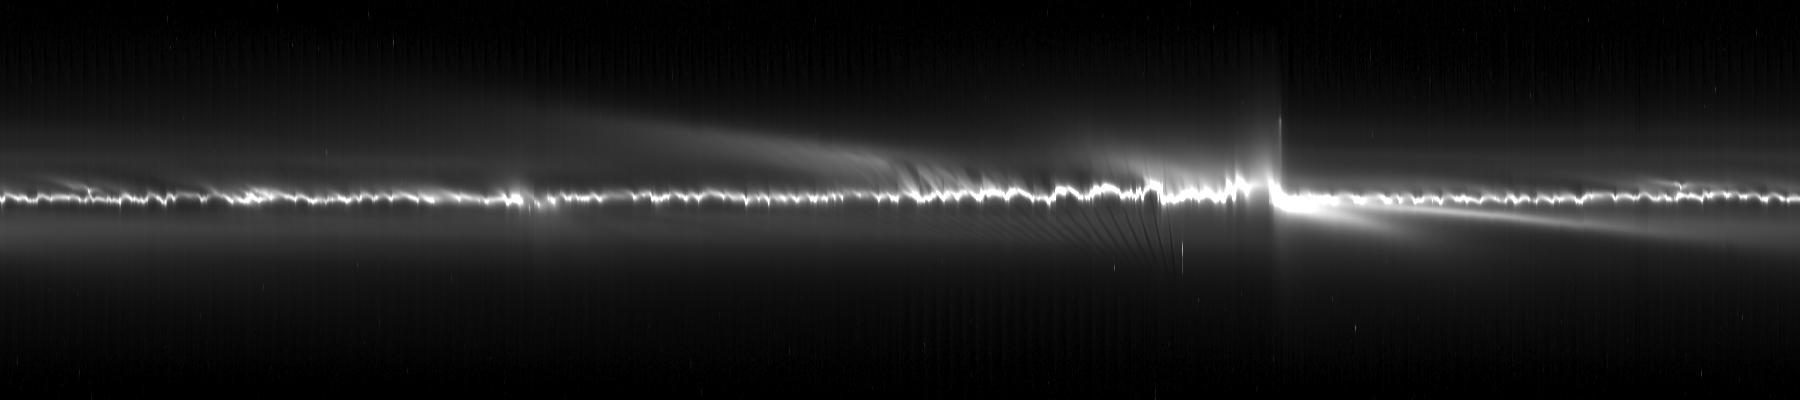
\includegraphics[width=\linewidth]{figures/fig1-fmovie-mosaic.png}
\caption{Mosaic of observation \code{iss\_\allowbreak{}039rf\_\allowbreak{}fmovie001\_\allowbreak{}vims}, a standard F movie taken as a rider on a VIMS-prime observation.}
\label{fig:fmovie-mosaic}
\end{figure}

\begin{figure}[tbp]
\centering
\noindent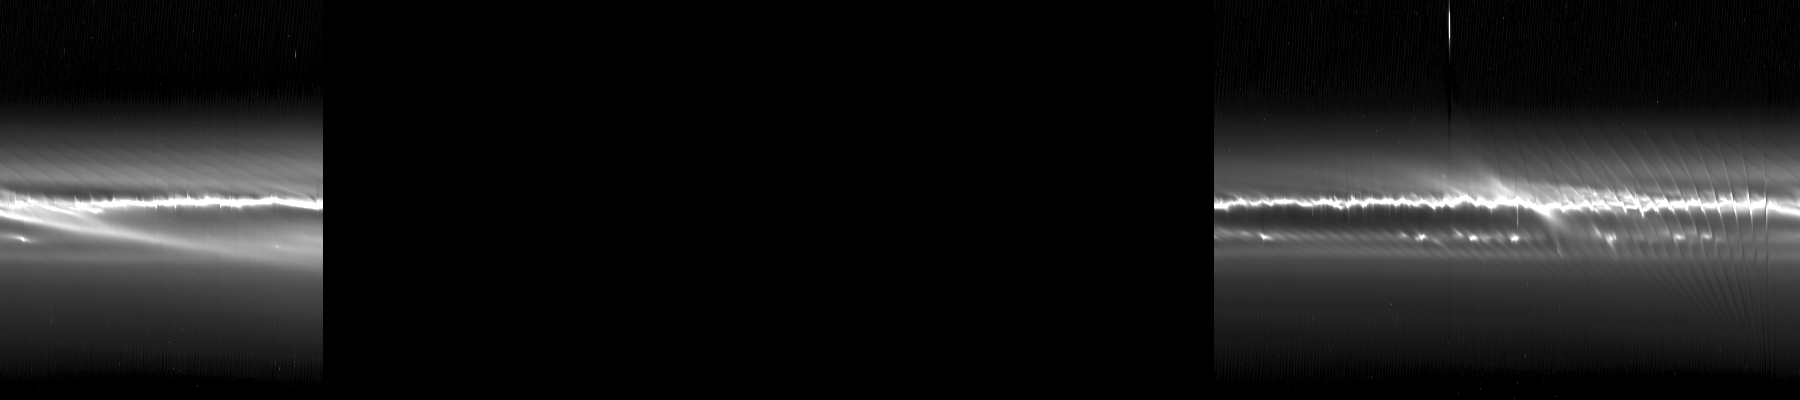
\includegraphics[width=\linewidth]{figures/fig2a-paired-mosaic-1.png}\\[2pt]
\noindent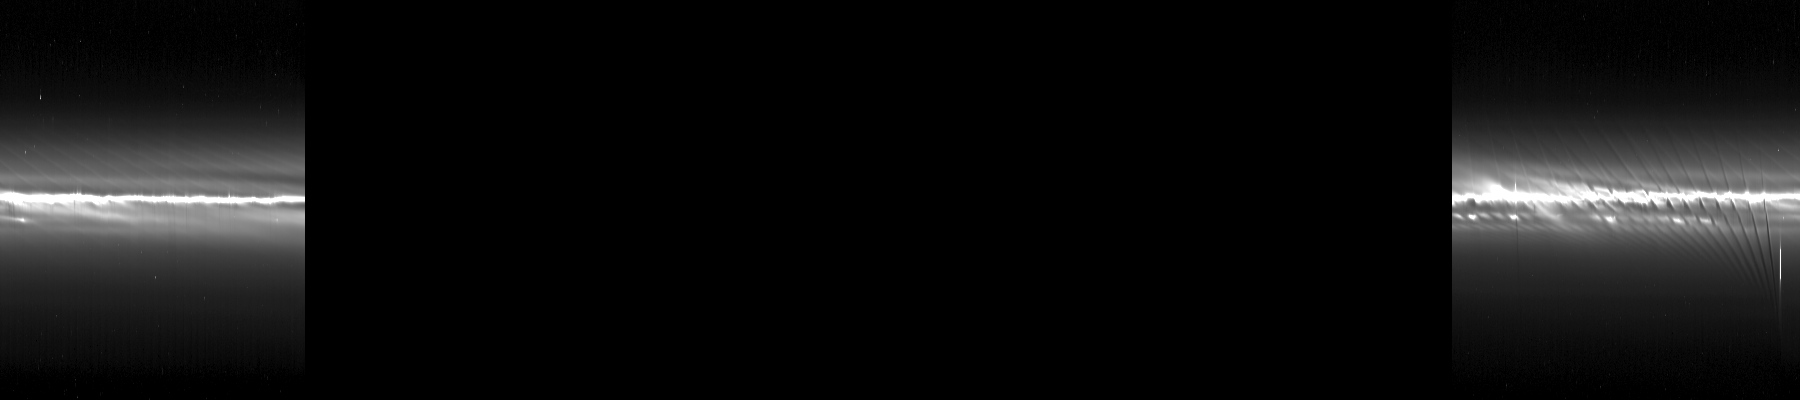
\includegraphics[width=\linewidth]{figures/fig2b-paired-mosaic-2.png}
\caption{Mosaics of observations \code{iss\_\allowbreak{}112rf\_\allowbreak{}fmovie002\_\allowbreak{}prime\_\allowbreak{}1} (top) and \code{iss\_\allowbreak{}112rf\_\allowbreak{}fmovie002\_\allowbreak{}prime\_\allowbreak{}2} (bottom). They cover approximately the same range of corotating longitudes but were taken at inertial longitudes roughly 180° apart. Morphological differences between the two are visible, giving potential insight into the orbits of the particles in these regions. (Flag M2.)}
\label{fig:paired-mosaics}
\end{figure}

\begin{figure}[tbp]
\centering
\noindent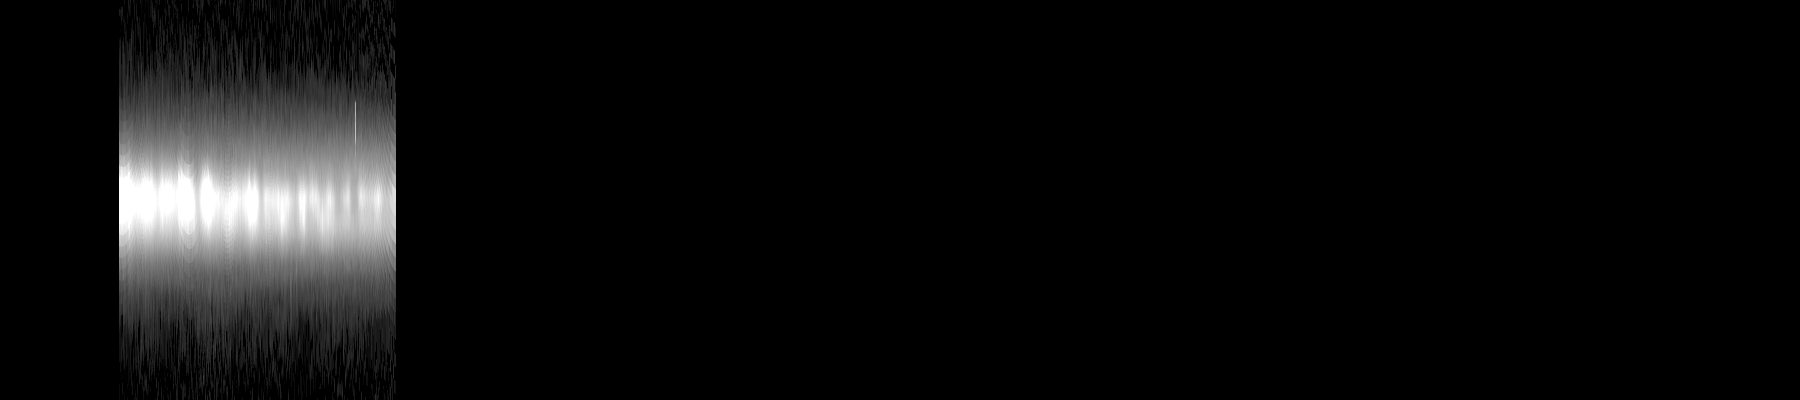
\includegraphics[width=\linewidth]{figures/fig3a-m3-mosaic-1.png}\\[2pt]
\noindent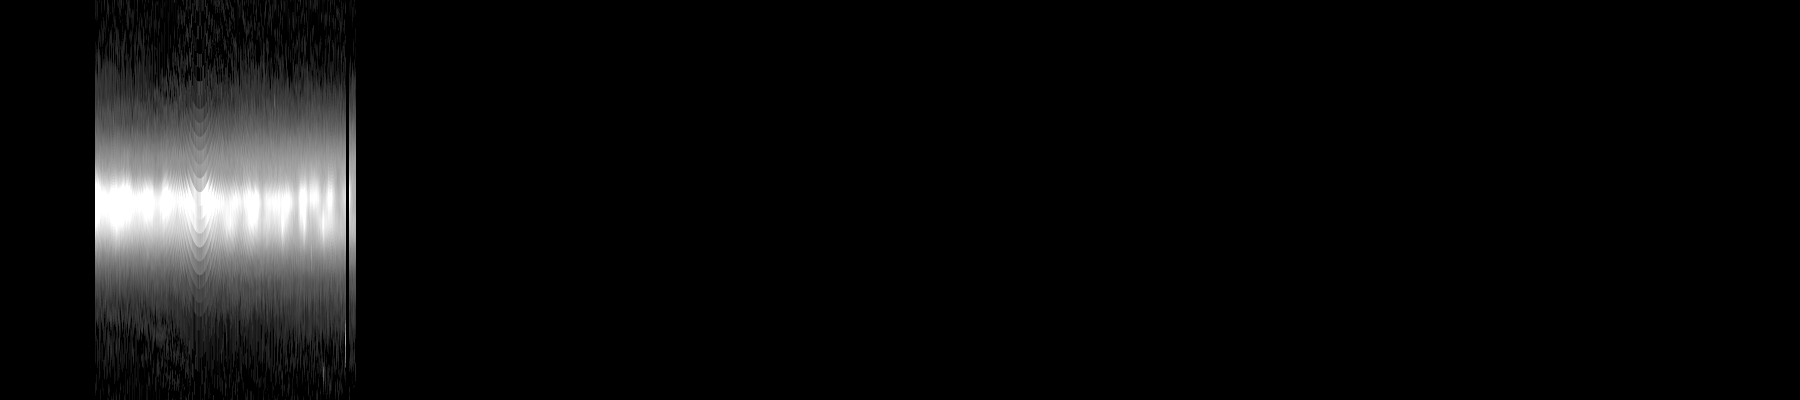
\includegraphics[width=\linewidth]{figures/fig3b-m3-mosaic-2.png}\\[2pt]
\noindent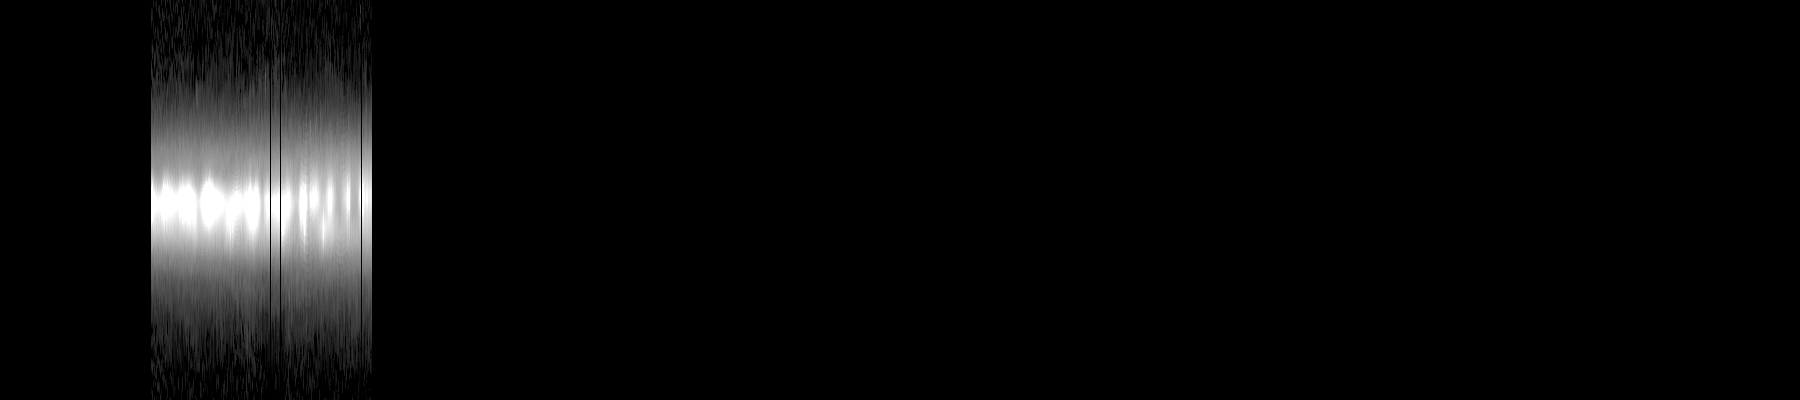
\includegraphics[width=\linewidth]{figures/fig3c-m3-mosaic-3.png}
\caption{A series of observations covering the same corotating longitudes but taken at successively increasing inertial longitudes. \code{iss\_\allowbreak{}105ri\_\allowbreak{}tmapn45lp001\_\allowbreak{}cirs\_\allowbreak{}1} (top) was taken at 78°–130°; \code{iss\_\allowbreak{}105ri\_\allowbreak{}tmapn45lp001\_\allowbreak{}cirs\_\allowbreak{}2} (middle) at 109°–154°; \code{iss\_\allowbreak{}105ri\_\allowbreak{}tmapn45lp001\_\allowbreak{}cirs\_\allowbreak{}3} (bottom) at 136°–186°. (Flag M3.)}
\label{fig:m3-mosaics}
\end{figure}

\begin{figure}[tbp]
\centering
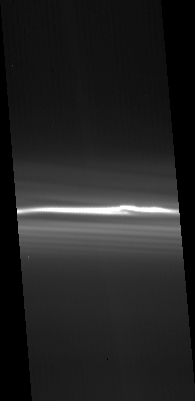
\includegraphics[width=0.327\linewidth]{figures/fig4a-reproj-img-1.png}
\hfill
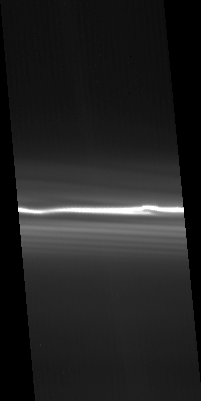
\includegraphics[width=0.327\linewidth]{figures/fig4b-reproj-img-2.png}
\hfill
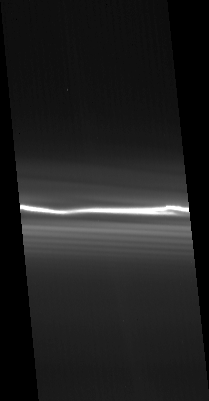
\includegraphics[width=0.327\linewidth]{figures/fig4c-reproj-img-3.png}
\caption{Three reprojected images from mosaic \code{iss\_\allowbreak{}191rf\_\allowbreak{}fmovie001\_\allowbreak{}prime\_\allowbreak{}1}, each covering approximately the same 4° range of corotating longitude. Source image index 0, \code{1748745661n} (left), was taken at inertial longitudes 5.7°–9.6°; index 4, \code{1748746261n} (middle), at 9.3°–13.3°; index 8, \code{1748746865n} (right), at 12.9°–17.1°. (Flag R.)}
\label{fig:r-reproj-imgs}
\end{figure}

\begin{figure}[tbp]
\centering
\noindent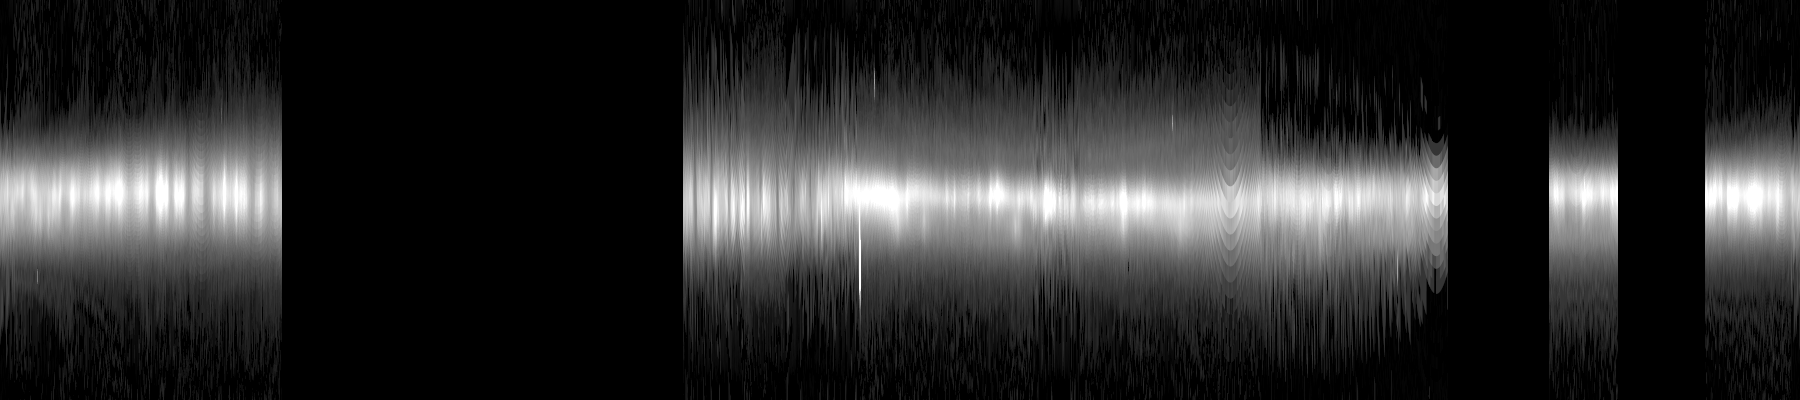
\includegraphics[width=\linewidth]{figures/fig5-non-corot-mosaic.png}
\caption{Non-inertial, non-corotating mosaic \code{iss\_\allowbreak{}098ri\_\allowbreak{}tmapn30lp001\_\allowbreak{}cirs}, which covers most of the full corotating range 0°–359.98°, taken from inertial longitudes 93°–309°. (Flag N.)}
\label{fig:non-corot-mosaic}
\end{figure}

\clearpage

\subsection{Calibration}
\label{sec:calibration}

Calibrated images were retrieved from the PDS Ring-Moon Systems Node archive\footnote{\href{https://pds-rings.seti.org/holdings/calibrated/COISS_2xxx/}{https://pds-rings.seti.org/holdings/calibrated/COISS\_\allowbreak{}2xxx/}}. Each image was calibrated by the Node using the CISSCAL 4.0 pipeline \zcite{(Knowles 2018)} into units of I/F\footnote{I/F is a dimensionless value that gives the ratio of the observed intensity to the incoming flux from the light source, assuming a perfect Lambert surface illuminated at normal incidence. See French et al. \zcite{(2012)} for more details.}. At the time of writing, the calibrated files are being migrated to the PDS4 standard, and they will be archived as collections within the \code{cassini\_\allowbreak{}iss\_\allowbreak{}cruise} and \code{cassini\_\allowbreak{}iss\_\allowbreak{}saturn} bundles.\footnote{\href{https://pds-rings.seti.org/pds4/bundles/cassini_iss}{https://pds-rings.seti.org/pds4/bundles/cassini\_\allowbreak{}iss}}


\subsection{Navigation}
\label{sec:navigation}

The spacecraft pointing information present in SPICE C kernels is known to have errors on the order of dozens of NAC pixels. Before processing each image, an automatic navigation procedure \zcite{(French et al. 2014b, 2016)} was performed that matched the image with features predicted to be present in it, such as stars and the edge of the A ring. Once a mosaic was created from a set of images, the quality of the navigation was evaluated by eye and, in some cases, the navigation of some images was manually adjusted for the best visual result. The (automatically or manually) adjusted C matrix for each image is reported in a supplemental file called \code{IMGID\_\allowbreak{}reproj\_\allowbreak{}img\_\allowbreak{}suppl.\allowbreak{}txt} in the \code{data\_\allowbreak{}reproj\_\allowbreak{}img} collection. See Section~\ref{sec:data-reproj-img}.

The outcome of that visual evaluation is recorded for each mosaic in the \code{nav\_\allowbreak{}quality} field of the mosaic label and the global index files (Section~\ref{sec:the-global-index-files}). The grade is subjective and describes the mosaic as a whole:

\begin{itemize}
\item \textbf{G} (good): the ring core runs continuously across the mosaic, with no visible radial step or tilt where one source image abuts the next.
\item \textbf{F} (fair): small radial steps or tilts are visible at some image boundaries, but the core is unambiguous at every longitude and photometry is not noticeably affected.
\item \textbf{P} (poor): at least one source image is misregistered enough to displace the core visibly. The mosaic remains usable for many purposes, but measurements at the affected longitudes should be treated with caution.
\end{itemize}

Because the grade covers the whole mosaic, a mosaic graded \textbf{F} or \textbf{P} may still contain a majority of well-navigated images.


\subsection{Reprojection}
\label{sec:reprojection}

Each calibrated image was converted to a reprojected image by mapping the pixels in the source image onto a two-dimensional grid with corotating longitude on the X axis and distance from the nominal F ring core (Δ\textit{r}) on the Y axis.


\subsubsection{F ring orbit}
\label{sec:f-ring-orbit}

Various orbital fits for the F ring core have been developed over time \zcite{(Albers et al. 2012; Cooper et al. 2013; Cuzzi et al. 2024)}. We use the orbit fit from Albers et al. \zcite{(2012)}, Table 3, fit 2, throughout:

\begin{equation*}
\begin{aligned}
n &= 581.964^{\circ}\,\mathrm{/day} & a &= 140{,}221.3\ \mathrm{km} & e &= 0.00235 \\
\varpi_{0} &= 24.2^{\circ} & \dot{\varpi} &= 2.70025^{\circ}\,\mathrm{/day} \\
\Omega_{0} &= 15.0^{\circ} & \dot{\Omega} &= -2.68778^{\circ}\,\mathrm{/day}
\end{aligned}
\end{equation*}

The angles $\varpi_{0}$ and $\Omega_{0}$ are the values at $\mathit{ET} = 0$, the J2000 epoch (2000-01-01T12:00:00 Barycentric Dynamical Time, TDB), where \textit{ET} is the ephemeris time SPICE reports; the rates $\dot{\varpi}$ and $\dot{\Omega}$ carry them forward to the time of each observation, as in the core radius formula below. This epoch is separate from the corotation epoch defined below, which is used only to relate corotating and inertial longitude.

Inertial ring longitude is measured from the reference direction — the ascending node of Saturn’s equatorial plane on the Earth’s mean equator of J2000 — in the direction of orbital motion along that plane to the ring’s ascending node, and thence along the ring plane.

Corotating longitude is based on a reference frame that rotates with the mean motion of the F ring. We use 2007-01-01T00:00:00Z as the epoch when corotating longitude and inertial longitude are equal. To convert from inertial to corotating longitude:

\begin{equation*}\mathit{corot} = \left(\mathit{inertial} - n\,\frac{\mathit{ET} - \mathit{epoch\_ET}}{86400}\right) \bmod 360\end{equation*}

and to convert from corotating to inertial longitude:

\begin{equation*}\mathit{inertial} = \left(\mathit{corot} + n\,\frac{\mathit{ET} - \mathit{epoch\_ET}}{86400}\right) \bmod 360\end{equation*}

where \textit{ET} is the ephemeris (SPICE) time of the image in seconds and \textit{epoch\_\allowbreak{}ET} is the corotating epoch in seconds, equal to 220881665.1839181.

Note that the choice of epoch is arbitrary, and when comparing absolute corotating longitudes from different sources it is important to convert them to a common reference frame. For example, Murray et al. \zcite{(2008)} used 2007-01-01T12:00:00Z and French et al. \zcite{(2012)} used 2004-01-01T12:00:00Z, while French et al. \zcite{(2014a)} used the same epoch adopted here.

To determine the radius of the F ring core, we use the standard formula:

\begin{equation*}r_{\mathrm{core}}=\frac{a(1-e^{2})}{1+e\cos\left(\lambda-\left(\varpi_{0}+\dot{\varpi}\frac{\mathit{ET}}{86400}\right)\right)}\end{equation*}

where \textit{λ} is the inertial longitude (converted from the corotating longitude as described above), so that the argument of the cosine is the true anomaly.


\subsubsection{Reprojection process}
\label{sec:reprojection-process}

The reprojection grid runs from 0° to 359.98° in steps of 0.02° ($\sim$49 km) for corotating longitude (18,000 pixels), and −1000 km to +1000 km in steps of 5 km for Δ\textit{r} (401 pixels). This gives an aspect ratio of roughly 10:1. For each corotating longitude, the radius is relative to the absolute radius of the core at the associated inertial longitude and time. This means that, while the core of the F ring varies in radius from 139,892 km to 140,551 km throughout its orbit, the core in the reprojected image will always look like an approximately straight line at $\Delta r = 0$, corresponding to Y = 200. Note that the odd number of pixels on the Y axis provides an equal number of radii on either side of the core, with the predicted core precisely in the center.

As the majority of reprojected images cover only a few degrees of corotating longitude, archiving files of the complete 18,000 × 401 grid would be extremely wasteful. As a result, the reprojected image data products are clipped on the X axis to the minimum and maximum corotating longitudes that contain valid data; see the associated label for information on these values. In the case where the extent of a reprojected image wraps around from 359.98° to 0°, the minimum corotating longitude is larger than the maximum corotating longitude, and the reprojected image is stored in two sections, first from the minimum corotating longitude to 359.98° and then from 0° to the maximum corotating longitude. See Section~\ref{sec:data-reproj-img} for the formulas that map a longitude to a column in this case. In all cases, if there is missing data within the remaining grid (either due to insufficient radial extent available in the source image, or discontinuous corotating longitudes), it is marked with the sentinel value −999.

During the reprojection process, several other parameters are computed for each corotating longitude, as the mean over that radial slice:

\begin{itemize}
\item Phase angle (°)
\item Emission angle (°)
\item Incidence angle (°)
\item Radial resolution (km/pixel)
\item Longitudinal resolution (°/pixel)
\end{itemize}
Following standard planetary ring practice, incidence and emission angles are measured from the ring-plane normal on the sunlit side. The incidence angle is therefore always below 90°, and an emission angle below 90° means the ring is being viewed from its lit side.

These values are reported in a table \code{IMGID\_\allowbreak{}reproj\_\allowbreak{}img\_\allowbreak{}metadata\_\allowbreak{}params.\allowbreak{}tab} (Section~\ref{sec:data-reproj-img}) that is associated with each reprojected image. Other parameters describing the orbits of the F ring, Prometheus, and Pandora at the time of the source image are included as well:

\begin{itemize}
\item Core Radius (distance from Saturn in km, computed using the formula above)
\item Longitude of Ascending Node (°)
\item Longitude of Pericenter (°)
\item True Anomaly (°)
\item Corotating Longitude of Prometheus (°) in the same corotating frame used for the F ring
\item Radius (distance from Saturn) of Prometheus (km)
\item Corotating Longitude of Pandora (°) in the same corotating frame used for the F ring
\item Radius (distance from Saturn) of Pandora (km)
\end{itemize}
The positions of Prometheus and Pandora were computed with SPICE, taking the satellite positions from the Saturn system ephemeris \code{sat393.\allowbreak{}bsp}, planetary positions from \code{de438.\allowbreak{}bsp}, and the ring-plane orientation from the planetary constants kernel \code{pck00010\_\allowbreak{}edit\_\allowbreak{}v01.\allowbreak{}tpc}. The metakernel archived in this bundle’s \code{spice\_\allowbreak{}kernels} collection (Section~\ref{sec:the-spice-kernels-directory}) lists every kernel used anywhere in the production of this bundle, which is a larger set than these three.

Mean, minimum, and maximum values for many of these parameters are included in the label for each reprojected image as well. See Section~\ref{sec:reprojected-image-and-mosaic-metadata-params} for a complete list of the metadata parameters provided.


\subsection{Mosaic creation}
\label{sec:mosaic-creation}

Mosaics were created by stitching together one or more reprojected images. The resulting grid for a mosaic is the same 18,000 × 401 pixel grid as used for each reprojected image (Section~\ref{sec:reprojection}). For each corotating longitude in the mosaic, the entire radial stripe is taken from a single image. The image is chosen first based on which image has the most valid pixels at that corotating longitude; when there is a tie, the image with the smallest mean radial resolution is used. This guarantees that the resulting mosaic will have the most data and the highest resolution possible, but does not guarantee that the selected reprojected images will change monotonically with corotating longitude. This can result in a slight temporal “blurring” across small ranges of corotating longitude.

As with reprojected images, several parameters are stored for each corotating longitude and provided in a table file \code{OBSID\_\allowbreak{}mosaic\_\allowbreak{}metadata\_\allowbreak{}params.\allowbreak{}tab} (Section~\ref{sec:data-mosaic-and-data-mosaic-bkg-sub}) associated with each mosaic:

\begin{itemize}
\item Source reprojected image number
\item SPICE ET of source image
\item Mean phase angle (°)
\item Mean emission angle (°)
\item Incidence angle (°)
\item Mean radial resolution (km/pixel)
\item Mean longitudinal resolution (°/pixel)
\item Core Radius (distance from Saturn in km, computed using the formula above)
\item Longitude of Ascending Node (°)
\item Longitude of Pericenter (°)
\item True Anomaly (°)
\item Corotating Longitude of Prometheus (°) in the same corotating frame used for the F ring
\item Radius (distance from Saturn) of Prometheus (km)
\item Corotating Longitude of Pandora (°) in the same corotating frame used for the F ring
\item Radius (distance from Saturn) of Pandora (km)
\end{itemize}
Mean, minimum, and maximum values for many of these parameters are included in the label for each mosaic as well. See Section~\ref{sec:reprojected-image-and-mosaic-metadata-params} for a complete list of the metadata parameters provided.


\subsection{Background modeling}
\label{sec:background-modeling}

The final step in the data production pipeline is modeling and subtracting the background gradient for each mosaic. The background gradient is modeled separately for each corotating longitude using a linear function. Regions normally consisting of the innermost 50 rows ($\Delta r$ = −1000 to −755 km) and the outermost 51 rows ($\Delta r$ = +750 to +1000 km) are used to fit a linear model, which is then subtracted from the complete 401-row radial slice. When creating the model, pixel values that are statistically anomalous compared to nearby longitudes are automatically masked. This removes stars, Prometheus and Pandora, and bad pixels from the background model computation. In some cases, the standard range of 50 pixels on each side is not appropriate. Reasons include large objects such as Prometheus covering the entire 50-row range, the reprojected source images not providing data for the entire radial range (which would require the background margins to be increased in size), and very low-resolution images where the F ring bleeds over into the background region (which would require background margins to be reduced). Such determinations were made through careful examination of each mosaic and the extent of the background margin was manually adjusted as needed. Whenever possible, the new margins were chosen to have minimal effect on computation of equivalent width.\footnote{Equivalent width is a photometric value that integrates the brightness of a radial slice, taking into account the resolution of the image.} The chosen margins are reported in the label for each background-subtracted mosaic and in the \code{bkgnd\_\allowbreak{}lower\_\allowbreak{}limit} and \code{bkgnd\_\allowbreak{}upper\_\allowbreak{}limit} fields of the global index file (Section~\ref{sec:the-global-index-files}). Both are signed values of Δ\textit{r} in km, so that the interior background region runs from −1000 km out to \code{bkgnd\_\allowbreak{}lower\_\allowbreak{}limit} (normally −750 km) and the exterior region runs from \code{bkgnd\_\allowbreak{}upper\_\allowbreak{}limit} (normally +750 km) out to +1000 km.

In cases where, even after adjusting the margins, there was insufficient radial data to create a background model for some longitudes, those longitudes were marked as invalid and deleted from the background-subtracted mosaic. As a result, the background-subtracted mosaic may have fewer (and sometimes substantially fewer) valid longitudes than the original mosaic. An example is shown in Figure~\ref{fig:bkg-sub-mosaic}.

The model is fit to noisy data, so subtracting it leaves the background regions scattered about zero. Roughly half of the pixels away from the ring in a background-subtracted mosaic are consequently negative. This is expected. Keep these values instead of clipping them at zero; discarding the negative half of the noise biases any integral over a radial slice, equivalent width included.

Each background-subtracted mosaic was inspected and the result recorded in the \code{bkgnd\_\allowbreak{}quality} field of the label and the global index file (Section~\ref{sec:the-global-index-files}). Like \code{nav\_\allowbreak{}quality} (Section~\ref{sec:navigation}), the grade is subjective:

\begin{itemize}
\item \textbf{G} (good): the regions away from the ring are flat after subtraction at essentially all longitudes.
\item \textbf{F} (fair): a residual gradient or offset remains at some longitudes, small enough that equivalent widths are still usable.
\item \textbf{P} (poor): the model is visibly wrong over a substantial range of longitudes, usually because too little background data was available or because the F ring dust sheet extends into the background region.
\end{itemize}

\begin{figure}[tbp]
\centering
\noindent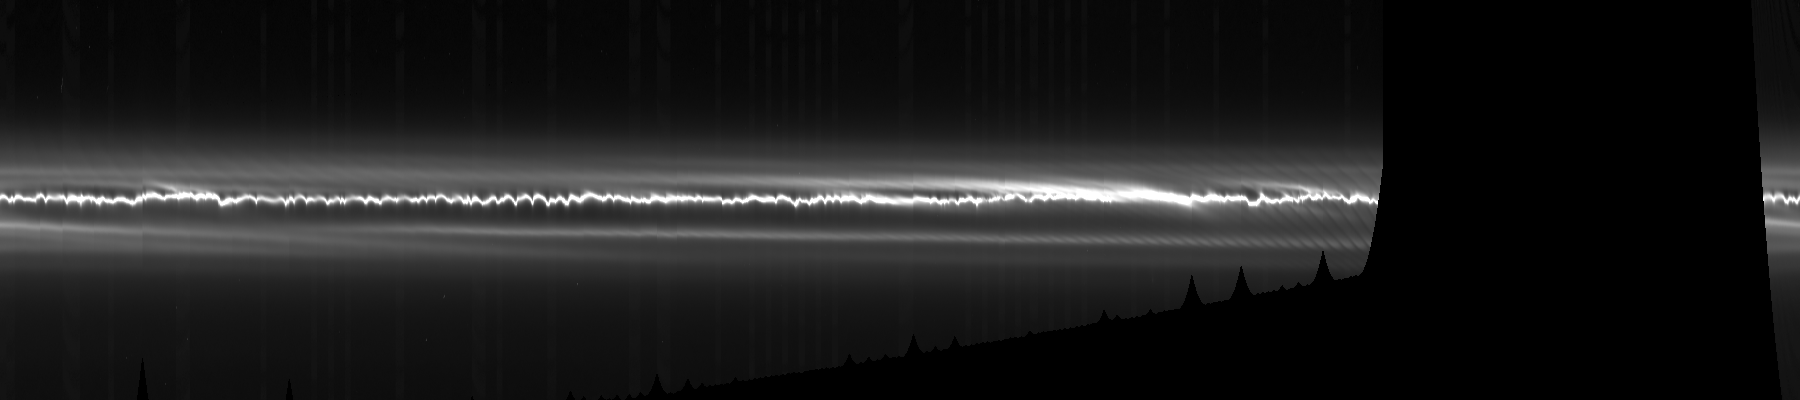
\includegraphics[width=\linewidth]{figures/fig6a-mosaic-original.png}\\[2pt]
\noindent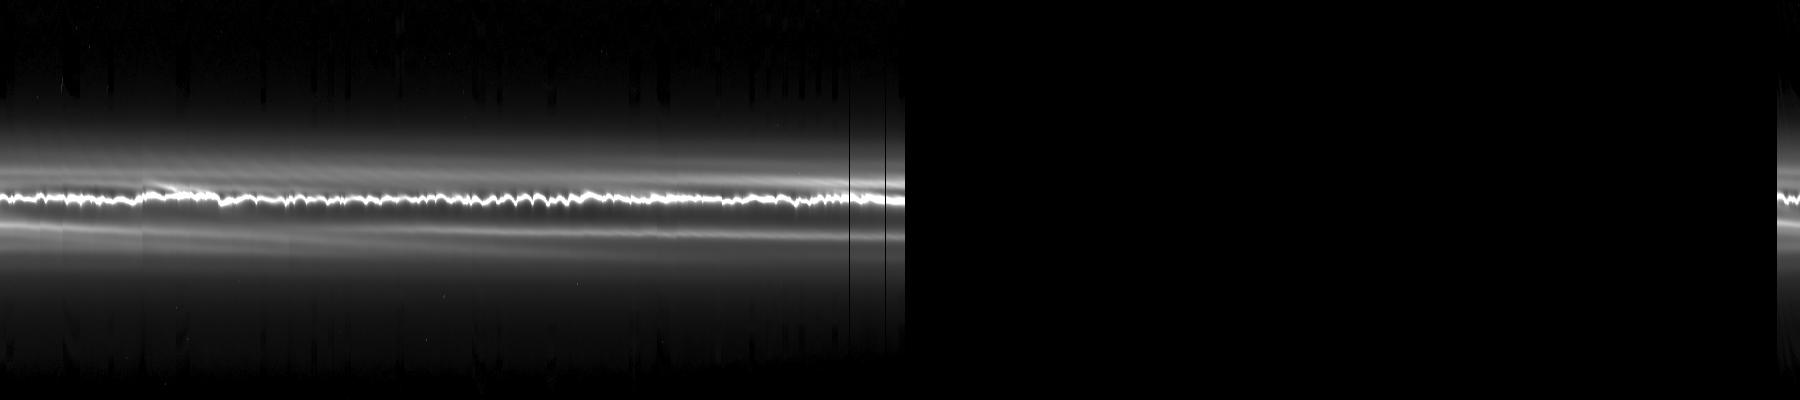
\includegraphics[width=\linewidth]{figures/fig6b-mosaic-bkg-sub.png}
\caption{Original mosaic iss\_\allowbreak{}007ri\_\allowbreak{}hpmrdfmov001\_\allowbreak{}prime (top) and associated background-subtracted mosaic (bottom). The lack of some data in the original mosaic (to the lower left of the large blank area) prevents the creation of a background model for those longitudes, resulting in a background-subtracted mosaic with substantially fewer valid longitudes.}
\label{fig:bkg-sub-mosaic}
\end{figure}

\clearpage
% Section 4: Bundle organization and directory structure

\section{Bundle organization and directory structure}
\label{sec:bundle-organization-and-directory-structure}

The Cassini ISS F Ring Mosaics \textit{bundle} is organized in a hierarchical directory structure, with each directory containing a PDS4 \textit{collection} of a different type of \textit{product}.\footnote{Refer to the documents in Section~\ref{sec:pds4-standards-and-documentation} for further information on the PDS4 concepts of \textit{bundle}, \textit{collection}, and \textit{data product}.} There are data and browse collections for reprojected images, mosaics and background-subtracted mosaics, plus collections for documentation, miscellaneous files (the global index files), context products, SPICE kernels and XML schemas. The top-level directory structure is:

\begin{CodeBlock}
cassini_iss_fring_mosaics_rsfrench2025/
├── bundle.lblx
├── readme.txt
├── browse_mosaic/
├── browse_mosaic_bkg_sub/
├── browse_reproj_img/
├── context/
├── data_mosaic/
├── data_mosaic_bkg_sub/
├── data_reproj_img/
├── document/
├── miscellaneous/
├── spice_kernels/
└── xml_schema/
\end{CodeBlock}

Each directory is described in the sections below. The \code{context} and \code{xml\_\allowbreak{}schema} directories are used internally by PDS and will not be discussed further.

For reference, the following types of data products and support files are available:

\begin{itemize}
\item \textbf{Reprojected images:} These files contain rectangular reprojections of calibrated image files. Like the calibrated files, they are in units of I/F. Associated table files provide information about each longitude. These files are in the \code{data\_\allowbreak{}reproj\_\allowbreak{}img} directory. See Section~\ref{sec:data-reproj-img}.
\item \textbf{Mosaics:} These files contain mosaics stitched together from multiple reprojected images. Like the reprojected images, they are in units of I/F. Associated table files provide information about each longitude. These files are in the \code{data\_\allowbreak{}mosaic} directory. See Section~\ref{sec:data-mosaic-and-data-mosaic-bkg-sub}.
\item \textbf{Background-subtracted mosaics:} These files contain the same mosaics as above, but each mosaic has had a linear background model subtracted for each longitude. They are in units of I/F. Associated table files provide information about each longitude. These files are in the \code{data\_\allowbreak{}mosaic\_\allowbreak{}bkg\_\allowbreak{}sub} directory. See Section~\ref{sec:data-mosaic-and-data-mosaic-bkg-sub}.
\item \textbf{Browse images:} Browse images in four sizes are available for each of the reprojected images, mosaics, and background-subtracted mosaics. These are \textit{not} meant for scientific analysis and are only meant for visual examination of the contents of the data file. The original I/F data has been mapped to integers from 0 to 255 and non-linearly stretched to make dim features easier to see. The stretch uses a blackpoint at the minimum valid value or zero, whichever is greater, a whitepoint at the 99.8th-percentile value, and a gamma of 0.5. Because the blackpoint is never negative, negative values are all shown as black. These files are in the three \code{browse\_\allowbreak{}*} directories. See Sections~\ref{sec:browse-reproj-img} and \ref{sec:browse-mosaic-and-browse-mosaic-bkg-sub}.
\item \textbf{Documentation:} This \textit{User Guide} is available in PDF format in the \code{document} directory. See Section~\ref{sec:user-guide}.
\item \textbf{Global index files:} These files provide a list of all reprojected images and mosaics in the bundle, along with tabulated metadata for each. They allow for easy programmatic searching on fields such as date and viewing geometry. These files are in the \code{miscellaneous} directory. See Section~\ref{sec:the-global-index-files}.
\item \textbf{SPICE kernels:} A SPICE metakernel specifying the kernels that were used during navigation and data processing is provided in the \code{spice\_\allowbreak{}kernels} directory. These files are not expected to be needed by most scientific users. See Section~\ref{sec:the-spice-kernels-directory}.
\item \textbf{PDS4 support files:} These files are required by the PDS4 standard and contain information about the contents of the bundle directory. However, they are likely to be less useful to a scientist using the data in the bundle. These files include \code{bundle.\allowbreak{}lblx}, \code{collection\_\allowbreak{}*.\allowbreak{}csv}, \code{collection\_\allowbreak{}*.\allowbreak{}lblx}, and the contents of the \code{context} and \code{xml\_\allowbreak{}schema} directories.
\end{itemize}

\subsection{The top-level directory}
\label{sec:the-top-level-directory}

The top-level directory contains the following files:

\begin{itemize}
\item \code{bundle.\allowbreak{}lblx}: The PDS4 bundle label, providing the high-level description of the entire archive.
\item \code{readme.\allowbreak{}txt}: A text file directing the user to this \textit{User Guide}.
\end{itemize}

\subsection{The \textit{browse} and \textit{data} directories}
\label{sec:the-browse-and-data-directories}

For each derived data type — reprojected image (Sections~\ref{sec:data-reproj-img} and \ref{sec:browse-reproj-img}), mosaic (Sections~\ref{sec:data-mosaic-and-data-mosaic-bkg-sub} and \ref{sec:browse-mosaic-and-browse-mosaic-bkg-sub}), and background-subtracted mosaic (Sections~\ref{sec:data-mosaic-and-data-mosaic-bkg-sub} and \ref{sec:browse-mosaic-and-browse-mosaic-bkg-sub}) — there is a \code{browse} and a \code{data} directory. These directories have the same internal structure:

\begin{CodeBlock}
<dirname>/
├── collection_<dirname>.csv
├── collection_<dirname>.lblx
├── OBSID1/
├── OBSID2/
├── ...
└── OBSIDn/
\end{CodeBlock}

The \code{collection\_\allowbreak{}<dirname>.\allowbreak{}csv} file contains a list of all of the data products present for all OBSIDs in this directory, and the accompanying label describes its metadata. The data products themselves are separated by OBSID for ease of retrieval and to keep the number of files in each subdirectory relatively small. Throughout this guide, OBSID is the Cassini observation name converted to lowercase, including any numeric chunk suffix (Section~\ref{sec:image-selection}), and IMGID is the identifier of a single source image: its ten-digit Cassini spacecraft clock (SCLK) count followed by \code{n} for the Narrow Angle Camera or \code{w} for the Wide Angle Camera, as in \code{1622049830n}. IMGID is the key that links a reprojected product back to the original COISS image.

Each derived data type has its own file structure within each OBSID directory.


\subsubsection{data\_reproj\_img}
\label{sec:data-reproj-img}

This directory contains the individual reprojected images (Section~\ref{sec:reprojection}) organized by OBSID. The directory structure is:

\begin{CodeBlock}
data_reproj_img/
├── collection_data_reproj_img.csv
├── collection_data_reproj_img.lblx
├── OBSID1/
│   ├── IMGID1_reproj_img.lblx
│   ├── IMGID1_reproj_img.img
│   ├── IMGID1_reproj_img_metadata_params.tab
│   ├── IMGID1_reproj_img_suppl.txt
│   └── ...
└── ...
\end{CodeBlock}

The file \code{IMGID\_\allowbreak{}reproj\_\allowbreak{}img.\allowbreak{}lblx} contains all of the details about the reprojected image, including the reprojection and viewing geometry. Every excerpt in this section is taken from image \code{1622049830n} of observation \code{iss\_\allowbreak{}111rf\_\allowbreak{}fmovie002\_\allowbreak{}prime}:

\begin{CodeBlock}[fontsize=\scriptsize]
<rings:epoch_reprojection_basis_utc>2007-01-01T00:00:00.000Z</rings:epoch_reprojection_basis_utc>
<rings:reprojection_plane>Equator</rings:reprojection_plane>
<rings:corotating_flag>Y</rings:corotating_flag>
<rings:corotation_rate unit="deg/s">0.006735694444</rings:corotation_rate> <!-- 581.964 deg/day -->
<rings:mean_phase_angle unit="deg">34.334</rings:mean_phase_angle>
<rings:minimum_phase_angle unit="deg">34.208</rings:minimum_phase_angle>
<rings:maximum_phase_angle unit="deg">34.373</rings:maximum_phase_angle>
<rings:mean_incidence_angle unit="deg">88.824</rings:mean_incidence_angle>
<rings:minimum_incidence_angle unit="deg">88.824</rings:minimum_incidence_angle>
<rings:maximum_incidence_angle unit="deg">88.824</rings:maximum_incidence_angle>
<rings:mean_emission_angle unit="deg">103.117</rings:mean_emission_angle>
<rings:minimum_emission_angle unit="deg">102.901</rings:minimum_emission_angle>
<rings:maximum_emission_angle unit="deg">103.339</rings:maximum_emission_angle>
<rings:minimum_corotating_ring_longitude unit="deg">186.60</rings:minimum_corotating_ring_longitude>
<rings:maximum_corotating_ring_longitude unit="deg">199.56</rings:maximum_corotating_ring_longitude>
<rings:minimum_ring_radius unit="km">138896.295</rings:minimum_ring_radius>
<rings:maximum_ring_radius unit="km">140916.702</rings:maximum_ring_radius>
<rings:Reprojection_Grid_Parameters>
    <local_identifier>reproj_grid</local_identifier>
    <rings:reprojection_grid_radial_sampling_interval unit="km">5.0</rings:reprojection_grid_radial_sampling_interval>
    <rings:reprojection_grid_longitudinal_sampling_interval unit="deg">0.02</rings:reprojection_grid_longitudinal_sampling_interval>
    <rings:minimum_radial_resolution unit="km">5.613</rings:minimum_radial_resolution>
    <rings:maximum_radial_resolution unit="km">6.487</rings:maximum_radial_resolution>
    <rings:mean_radial_resolution unit="km">5.853</rings:mean_radial_resolution>
    <rings:minimum_longitudinal_resolution unit="deg">0.00963</rings:minimum_longitudinal_resolution>
    <rings:maximum_longitudinal_resolution unit="deg">0.01046</rings:maximum_longitudinal_resolution>
    <rings:mean_longitudinal_resolution unit="deg">0.01007</rings:mean_longitudinal_resolution>
</rings:Reprojection_Grid_Parameters>
\end{CodeBlock}

and the details of the image file, \code{IMGID\_\allowbreak{}reproj\_\allowbreak{}img.\allowbreak{}img}:

\begin{CodeBlock}[fontsize=\scriptsize]
<File_Area_Observational>
    <File>
        <file_name>1622049830n_reproj_img.img</file_name>
        <creation_date_time>2026-09-08T19:31:25Z</creation_date_time>
        <file_size unit="byte">1040996</file_size>
        <md5_checksum>3d19ed500563eab78063a95eb57cbdd1</md5_checksum>
    </File>
    <!-- The calibrated, reprojected single image -->
    <Array_2D_Image>
        <local_identifier>reproj_image</local_identifier>
        <offset unit="byte">0</offset>
        <axes>2</axes>
        <axis_index_order>Last Index Fastest</axis_index_order>
        <description>
            Line is the radial axis and Sample is the co-rotating longitude axis.
            Line 0 is the innermost row, at a delta radius of -1000 km from the
            F ring core, and the delta radius increases outward by 5 km per line,
            so that delta radius = -1000 + 5 * Line km and the modeled core lies
            at Line 200. Sample 0 is the minimum co-rotating longitude given by
            rings:minimum_corotating_ring_longitude and the longitude increases
            by 0.02 degrees per sample, wrapping through 360 degrees when the
            minimum is greater than the maximum.
        </description>
        <Element_Array>
            <data_type>IEEE754LSBSingle</data_type>
            <unit>I/F</unit>
        </Element_Array>
        <Axis_Array>
            <axis_name>Line</axis_name> <!-- vertical (delta radius) -->
            <elements>401</elements>
            <sequence_number>1</sequence_number>
        </Axis_Array>
        <Axis_Array>
            <axis_name>Sample</axis_name> <!-- horizontal (co-rotating longitude) -->
            <elements>649</elements>
            <sequence_number>2</sequence_number>
        </Axis_Array>
        <Special_Constants>
            <!-- Data was missing or corrupted in the original image (either because it was off
             the edge of the FOV or because of a transmission error resulting in a partial or
             corrupted image) -->
            <missing_constant>-999</missing_constant>
        </Special_Constants>
    </Array_2D_Image>
</File_Area_Observational>
\end{CodeBlock}

The image file is a pure binary file with no headers or record separators. Data is stored in LSB IEEE 754 single-precision (32-bit) floating-point format. The Y axis (Δ\textit{r}) always has size 401 (which covers the radial distance from the core of −1000 km to +1000 km in steps of 5 km). The array is stored with the Sample (longitude) index varying fastest — all longitudes at one radius, then the next radius — so that it reshapes directly to (401, \textit{N}) in row-major order. Line index 0 is the innermost row, at Δ\textit{r} = −1000 km, and Δ\textit{r} increases outward with the Line index, so that Δ\textit{r} = −1000 + 5 × \textit{Line} km and the predicted core lies at Line 200. The X axis (corotating longitude) has a variable size depending on the number of longitudes that contain valid data (see Section~\ref{sec:reprojection}). Any array elements that do not contain valid data will be marked with the value −999. See Section~\ref{sec:reading-labels-and-data-product-files} for information on how to read these files with software.

An associated metadata file, \code{IMGID\_\allowbreak{}reproj\_\allowbreak{}img\_\allowbreak{}metadata\_\allowbreak{}params.\allowbreak{}tab}, contains information about each \textit{valid} longitude. This table has the general format:

\begin{CodeBlock}[fontsize=\scriptsize]
rings:corotating_ring_longitude,rings:observed_event_tdb,rings:inertial_ring_longitude,rings:radial_resolution,rings:longitudinal_resolution,rings:incidence_angle,rings:phase_angle,rings:emission_angle,core_radius,longitude_ascending_node,longitude_pericenter,true_anomaly,corotating_longitude_prometheus,radius_prometheus,corotating_longitude_pandora,radius_pandora
186.60, 296628214.587, 272.212,    6.487,  0.00963,  88.824,  34.369, 103.339, 139916.702, 147.322, 294.690, 337.522, 274.743, 139453.621,  68.058, 141137.545
186.62, 296628214.587, 272.232,    6.484,  0.00963,  88.824,  34.369, 103.339, 139916.658, 147.322, 294.690, 337.542, 274.743, 139453.621,  68.058, 141137.545
186.64, 296628214.587, 272.252,    6.480,  0.00964,  88.824,  34.368, 103.338, 139916.614, 147.322, 294.690, 337.562, 274.743, 139453.621,  68.058, 141137.545
186.66, 296628214.587, 272.272,    6.477,  0.00964,  88.824,  34.368, 103.337, 139916.571, 147.322, 294.690, 337.582, 274.743, 139453.621,  68.058, 141137.545
186.68, 296628214.587, 272.292,    6.473,  0.00964,  88.824,  34.367, 103.337, 139916.527, 147.322, 294.690, 337.602, 274.743, 139453.621,  68.058, 141137.545
[...]
\end{CodeBlock}

where the rows are in ascending corotating-longitude order and cover only the longitudes that contain valid data. Because a reprojected image that wraps around at 360° is stored starting at its minimum corotating longitude and continuing through 360° to its maximum (see Section~\ref{sec:reprojection}), and because the image may retain sentinel-filled columns at longitudes with no valid data, the rows do \textit{not} necessarily correspond one-to-one, in sequence, to the X indices of the image array; to associate a row with an image column, use the corotating ring longitude field instead of the row position. The column holding a given corotating longitude is \code{col = round(((longitude − min\_\allowbreak{}corotating\_\allowbreak{}ring\_\allowbreak{}longitude) mod 360) / 0.\allowbreak{}02)}, and column \textit{c} holds longitude \code{(min\_\allowbreak{}corotating\_\allowbreak{}ring\_\allowbreak{}longitude + 0.\allowbreak{}02 × c) mod 360}; the modulo handles the wraparound case (Section~\ref{sec:reading-labels-and-data-product-files}). This table gives the actual corotating longitude for each row as well as additional useful information such as the inertial longitude, radial resolution, angular (longitudinal) resolution, phase angle, emission angle, and various orbital parameters. See Sections~\ref{sec:reprojection} and \ref{sec:metadata-and-global-index-file-fields} for details about these fields and Section~\ref{sec:reading-labels-and-data-product-files} for information on how to read these files with software.

Finally, a supplemental information file, \code{IMGID\_\allowbreak{}reproj\_\allowbreak{}img\_\allowbreak{}suppl.\allowbreak{}txt}, describes the navigation process and the derived pointing for the image (see Section~\ref{sec:navigation}):

\begin{CodeBlock}[fontsize=\scriptsize]
This file contains a C-matrix that describes the rotation from the J2000 reference
frame to the camera pointing based upon analysis of the contents of the image.

Source Data Product ID = 1622049830n_calib
Image Start Time (SCLK) = 1/1622049829.163
Image Start Time (UTC) = 2009-05-26T16:42:27.992Z
Image Mid Time (SCLK) = 1/1622049830.012
Image Mid Time (UTC) = 2009-05-26T16:42:28.402Z
Image Stop Time (SCLK) = 1/1622049830.118
Image Stop Time (UTC) = 2009-05-26T16:42:28.812Z
Trajectory Kernels Query Time = Observation mid time
Stellar Aberration Correction = No
Light Travel Time Correction = No
Navigation Type = Stars
Navigated Boresight RA = 142.804 deg (09h31m13.028s)
Navigated Boresight Dec = -11.8016 deg (-011d48m05.706s)
Navigated Boresight Roll = -44.9209 deg
C-Matrix =
   -0.3130222448   -0.6513481158   -0.6912038095
   -0.5422429512   -0.4749368367    0.6931144083
   -0.7797369147    0.5917606215   -0.2045231298
\end{CodeBlock}

This pointing information is only provided for archival completeness and is not expected to be used by most scientific users.


\subsubsection{browse\_reproj\_img}
\label{sec:browse-reproj-img}

This directory contains browse images for each reprojected image. The directory structure is:

\begin{CodeBlock}
browse_reproj_img/
├── collection_browse_reproj_img.csv
├── collection_browse_reproj_img.lblx
├── OBSID1/
│   ├── IMGID1_browse_reproj_img.lblx
│   ├── IMGID1_browse_reproj_img_full.png
│   ├── IMGID1_browse_reproj_img_med.png
│   ├── IMGID1_browse_reproj_img_small.png
│   ├── IMGID1_browse_reproj_img_thumb.png
│   └── ...
└── ...
\end{CodeBlock}

Four sizes of browse image are provided. All of them omit the longitudes that contain no data, so a discontinuous set of longitudes is drawn as adjacent, and the width they are derived from is the number of longitudes that do contain data. Call that width \textit{V}. “Full” images are \textit{V} or 800 pixels wide, whichever is greater, by 401 pixels high. “Med” images are \textit{V}/10 or 400 pixels wide, whichever is greater, by 400 pixels high. “Small” images are 200×200 and “Thumb” images are 100×100. Because most reprojected images are narrow, a typical Full image is stretched horizontally to reach the 800-pixel minimum and a typical Med image is 400 pixels wide. Every size other than Full is resampled. The Med, Small and Thumb images carry the observation and image name drawn in the upper left corner. All sizes are contrast-stretched to use the full available grayscale and are not calibrated for scientific use. Missing data is drawn in black.


\subsubsection{data\_mosaic and data\_mosaic\_bkg\_sub}
\label{sec:data-mosaic-and-data-mosaic-bkg-sub}

These directories have identical structure and contain the original and background-subtracted mosaics, respectively. The directory structures are:

\begin{CodeBlock}
data_mosaic/
├── collection_data_mosaic.csv
├── collection_data_mosaic.lblx
├── OBSID1/
│   ├── OBSID1_mosaic.lblx
│   ├── OBSID1_mosaic.img
│   ├── OBSID1_mosaic_metadata_params.tab
│   ├── OBSID1_mosaic_metadata_src_imgs.tab
│   └── ...
└── ...
\end{CodeBlock}

and:

\begin{CodeBlock}
data_mosaic_bkg_sub/
├── collection_data_mosaic_bkg_sub.csv
├── collection_data_mosaic_bkg_sub.lblx
├── OBSID1/
│   ├── OBSID1_mosaic_bkg_sub.lblx
│   ├── OBSID1_mosaic_bkg_sub.img
│   ├── OBSID1_mosaic_bkg_sub_metadata_params.tab
│   ├── OBSID1_mosaic_bkg_sub_metadata_src_imgs.tab
│   └── ...
└── ...
\end{CodeBlock}

The format of the \code{OBSID1\_\allowbreak{}mosaic[\_\allowbreak{}bkg\_\allowbreak{}sub].\allowbreak{}lblx} and \code{OBSID1\_\allowbreak{}mosaic[\_\allowbreak{}bkg\_\allowbreak{}sub].\allowbreak{}img }files is very similar to the corresponding \code{reproj\_\allowbreak{}img} files described earlier. The only difference is that the mosaic image files are always 401 × 18,000, since mosaic images are never clipped to include only valid data (see Sections~\ref{sec:mosaic-creation} and \ref{sec:data-reproj-img}).

The \code{OBSID1\_\allowbreak{}mosaic[\_\allowbreak{}bkg\_\allowbreak{}sub]\_\allowbreak{}metadata\_\allowbreak{}params.\allowbreak{}tab} file is also similar to the corresponding \code{reproj\_\allowbreak{}img} file, with the exception that it contains one additional column:

\begin{CodeBlock}[fontsize=\scriptsize]
rings:corotating_ring_longitude,image_index,rings:observed_event_tdb,rings:inertial_ring_longitude,rings:radial_resolution,rings:longitudinal_resolution,rings:incidence_angle,rings:phase_angle,rings:emission_angle,core_radius,longitude_ascending_node,longitude_pericenter,true_anomaly,corotating_longitude_prometheus,radius_prometheus,corotating_longitude_pandora,radius_pandora
  4.60,    8, 296602047.773, 273.960,    5.289,  0.03542,  88.824,  38.053,  93.478, 139911.390, 148.136, 293.872, 340.088, 273.628, 139319.213,  70.526, 142262.214
  4.62,    8, 296602047.773, 273.980,    5.286,  0.03542,  88.824,  38.053,  93.477, 139911.351, 148.136, 293.872, 340.108, 273.628, 139319.213,  70.526, 142262.214
  4.64,    8, 296602047.773, 274.000,    5.282,  0.03543,  88.824,  38.053,  93.477, 139911.312, 148.136, 293.872, 340.128, 273.628, 139319.213,  70.526, 142262.214
  4.66,    8, 296602047.773, 274.020,    5.279,  0.03543,  88.824,  38.053,  93.477, 139911.273, 148.136, 293.872, 340.148, 273.628, 139319.213,  70.526, 142262.214
  4.68,    8, 296602047.773, 274.040,    5.276,  0.03543,  88.824,  38.053,  93.477, 139911.234, 148.136, 293.872, 340.168, 273.628, 139319.213,  70.526, 142262.214
[...]
\end{CodeBlock}

The same caution about row position applies here, but the mapping is simpler. A mosaic is never clipped, so its 18,000 columns always span the full grid: column \textit{c} holds corotating longitude 0.02 × \textit{c} degrees, and the column holding a given longitude is \code{col = round(longitude / 0.\allowbreak{}02)}. The rows of the table, however, cover only the longitudes that contain valid data, so row \textit{i} of the table is generally not column \textit{i} of the image.

The new column is \code{image\_\allowbreak{}index}, which indicates which reprojected image was used to provide data for this particular corotating longitude. The number in the \code{image\_\allowbreak{}index} column references the file \code{OBSID1\_\allowbreak{}mosaic[\_\allowbreak{}bkg\_\allowbreak{}sub]\_\allowbreak{}metadata\_\allowbreak{}src\_\allowbreak{}imgs.\allowbreak{}tab}, which contains a list of the LIDVIDs of the reprojected images that were used to create this mosaic:

\begin{CodeBlock}[fontsize=\scriptsize]
image_index,LIDVID
   0, urn:nasa:pds:cassini_iss_fring_mosaics_rsfrench2025:data_reproj_img:1622022571n_reproj_img::1.0
   1, urn:nasa:pds:cassini_iss_fring_mosaics_rsfrench2025:data_reproj_img:1622022704n_reproj_img::1.0
   2, urn:nasa:pds:cassini_iss_fring_mosaics_rsfrench2025:data_reproj_img:1622022841n_reproj_img::1.0
[...]
\end{CodeBlock}

While all of these files are in fixed-width format for rapid reading with appropriate software, they can also be read as if they were CSV files by standard spreadsheet software. In this case you must specify that the file is delimited by commas.

See Sections~\ref{sec:reprojection}, \ref{sec:mosaic-creation}, and \ref{sec:metadata-and-global-index-file-fields} for details about these fields and Section~\ref{sec:reading-labels-and-data-product-files} for information on how to read these files with software.


\subsubsection{browse\_mosaic and browse\_mosaic\_bkg\_sub}
\label{sec:browse-mosaic-and-browse-mosaic-bkg-sub}

These directories contain browse images for the corresponding mosaics. Browse images are provided in four sizes:

\begin{itemize}
\item Thumb: 100×100 pixels
\item Small: 200×200 pixels
\item Med: 1800×400 pixels
\item Full: 18,000×401 pixels
\end{itemize}
Every size other than Full is resampled from the mosaic. The Med, Small and Thumb images carry the observation name drawn in the upper left corner. Each browse image is contrast-stretched to use the full available grayscale and is not calibrated for scientific use. Missing data in the mosaic is drawn in black.


\subsection{The \textit{document} directory}
\label{sec:the-document-directory}

This directory contains the document collection and has the structure:

\begin{CodeBlock}
document/
├── collection_document.csv
├── collection_document.lblx
└── user_guide/
    ├── display_reproj_img.py
    ├── f-ring-mosaics-user-guide.lblx
    ├── f-ring-mosaics-user-guide.pdf
    ├── find_prometheus_closest_approaches.py
    ├── mosaic_utils.py
    ├── plot_ews_df.py
    └── plot_ews_ma.py
\end{CodeBlock}


\subsubsection{user\_guide}
\label{sec:user-guide}

The \code{user\_\allowbreak{}guide} directory contains the \textit{User Guide} (this document) and example programs.


\subsection{The \textit{miscellaneous} directory: the global index files}
\label{sec:the-miscellaneous-directory-the-global-index-fil}

This directory contains the global index files and has the structure:

\begin{CodeBlock}
miscellaneous/
├── collection_miscellaneous.csv
├── collection_miscellaneous.lblx
├── global_mosaic_bkg_sub_index.lblx
├── global_mosaic_bkg_sub_index.tab
├── global_mosaic_index.lblx
├── global_mosaic_index.tab
├── global_reproj_img_index.lblx
└── global_reproj_img_index.tab
\end{CodeBlock}


\subsubsection{The global index files}
\label{sec:the-global-index-files}

The \code{miscellaneous} directory contains three global index files, one for reprojected images, one for mosaics and one for background-subtracted mosaics. Each contains summary information about every product in its collection. The provided information is extensive and is designed to be useful to researchers who want to search for images or mosaics meeting certain requirements.

The following notes may be present for each reprojected image and mosaic. If multiple notes are present, they are separated by a semicolon. Each note is also described in words in an XML comment inside the \code{Observation\_\allowbreak{}Area} of the mosaic label. Items in braces below are replaced by the observation name or by a computed value.

\begin{itemize}
\item M1: Because Cassini observed the same inertial longitudes for more than one orbit of the F ring during \{root\_\allowbreak{}obsid\}, we have split the observation into multiple chunks, each corresponding to one complete orbit of the F ring.
\item M2: Because observation \{root\_\allowbreak{}obsid\} consists of two distinct movies covering approximately the same corotating longitudes but taken at inertial longitudes roughly 180° apart, we have split the observation into two chunks.
\item M3: Because observation \{root\_\allowbreak{}obsid\} consists of multiple movies covering approximately the same corotating longitudes but taken at different inertial longitudes (not 180° apart), we have split the observation into multiple chunks.
\item M4: Because Cassini observed multiple distinct inertial and corotating longitudes during \{root\_\allowbreak{}obsid\}, each making its own movie, we have split the observation into multiple chunks.
\item B: This background-subtracted mosaic contains substantially fewer valid longitudes than the original mosaic due to insufficient data being available to create a background model.
\item C: Some source images contained corrupted or missing data that could not be repaired during the construction of the mosaic.
\item E: Some source images may have been overexposed and the data values clipped; use caution when using this mosaic for photometry.
\item O: The sequence of source images used to create this mosaic was designed to observe a stellar occultation of the F ring core. As such, a star is present in each source image and may appear in the mosaic multiple times depending on how the reprojected images were stitched together. In addition, the source images were taken at roughly the same corotating longitudes and thus have significant overlap in the mosaic. To fully explore the occultation, use the reprojected images.
\item R: During this time, Cassini followed one corotating longitude for \{total\_\allowbreak{}secs\} seconds (\{total\_\allowbreak{}hours\} hours) by observing multiple inertial longitudes covering the (possibly discontinuous) \{diff\_\allowbreak{}inertial\} degrees from \{min\_\allowbreak{}inertial\} to \{max\_\allowbreak{}inertial\}.
\item N: During this time, Cassini observed multiple corotating longitudes at multiple inertial longitudes for \{total\_secs\} seconds (\{total\_hours\} hours). The inertial longitudes covered the (possibly discontinuous) \{diff\_inertial\} degrees from \{min\_inertial\} to \{max\_inertial\}.
\end{itemize}

\subsection{The \textit{spice\_kernels} directory}
\label{sec:the-spice-kernels-directory}

This directory contains the SPICE kernel collection, which consists of a single SPICE metakernel \code{kernels.\allowbreak{}ker} listing all kernels used to process the data for this bundle (see Section~\ref{sec:spice-toolkit}). As with the supplemental files described in Section~\ref{sec:data-reproj-img}, these files are only provided for archival completeness and are not expected to be used by most scientific users.

\clearpage
% Section 5: Reading labels and data product files

\section{Reading labels and data product files}
\label{sec:reading-labels-and-data-product-files}


\subsection{Introduction}
\label{sec:introduction-2}

The files in this bundle are archived in PDS4 format. PDS4 has the following basic structure:

\begin{itemize}
\item A \textit{bundle} consists of one or more \textit{collections}
\item A \textit{collection} consists of one or more \textit{data products}
\item Each \textit{data product} is defined by PDS4 label (\code{.\allowbreak{}lblx}), which gives information about the data and also includes information about the additional associated files that contain the actual data. These data files may be binary or text and may be stored in a variety of formats.
\end{itemize}
A full discussion of the PDS4 format is beyond the scope of this document and readers are referred to the resources in Section \ref{sec:pds4-standards-and-documentation} for additional reading. However, we will endeavor to provide enough information here to allow reading of these various files for research purposes without comprehensive knowledge of the PDS4 standard.

Two types of software can be used to read PDS4 labels and data files: generic off-the-shelf software that doesn’t understand PDS4 concepts, and specific tools or programming libraries that understand PDS4 labels. We will start by discussing the former.


\subsection{Using off-the-shelf programs}
\label{sec:using-off-the-shelf-programs}

Label files (\code{.\allowbreak{}lblx}), table files (\code{.\allowbreak{}tab}), and CSV files (\code{.\allowbreak{}csv}) are standard text files that can be read with any text editor. However, while this is sufficient to give you an overview of the contents of the file, each file has a specific format designed to be read and parsed by specific types of programs, and this can be done without the need for PDS4-specific software. Using the correct program in the correct way will make using these files much easier and more productive.


\subsubsection{Label files}
\label{sec:label-files}

Label files are written in XML (eXtensible Markup Language), a hierarchical file format much like a nested outline. For the best results, the use of a text editor that understands XML is helpful. Such an editor will likely have two main features:

\begin{itemize}
\item The ability to collapse and expand different levels of the hierarchy, so as to hide parts of the label that aren’t needed for the task at hand; and
\item Syntax coloring, where the open and close tags (\code{<tagname>data</\allowbreak{}tagname>}) are color-coded for ease of identification.
\end{itemize}
As text editors are constantly coming in and out of favor and are platform-specific, we will not recommend specific tools here. However, almost every sophisticated editor or programming IDE (Integrated Development Environment) either natively supports XML or has an XML plugin. In most cases the editor will automatically recognize the file as being in XML format, but in some cases it might be necessary to explicitly invoke the XML mode if the editor relies on the file extension (since \code{.\allowbreak{}lblx} is not a normal XML extension).


\subsubsection{Table files}
\label{sec:table-files}

Files with the extension \code{.\allowbreak{}tab} (including the metadata parameters, source image index, and global indexes) are formatted as \textit{fixed-width comma-delimited tables}. That is, they look like:

\begin{CodeBlock}
Value123   ,ValueA  ,ValueB
Value45678 ,ValueCDE,ValueF
\end{CodeBlock}

This format allows software that knows the width of each column to efficiently read the table (see below), but simultaneously permits reading by the wide range of software that supports comma-separated value (CSV) files, such as spreadsheet programs. In this case, when opening the table file, you may find that the program identifies the table as fixed-width. Unfortunately, in this case, it will end up adding the comma to each field. To properly read a table in a spreadsheet program, be sure to specify that the file is “delimited” and that the delimiter is “,”; also specify that you want whitespace stripped if possible.


\subsubsection{CSV files}
\label{sec:csv-files}

Files with the extension \code{.\allowbreak{}csv} (mainly the collection files) are formatted as \textit{variable-width comma-separated value} files. These files can be read the same way as the above table files, except it is more likely programs will correctly identify them as delimited instead of fixed width from the beginning.


\subsubsection{Image files}
\label{sec:image-files}

Files with the extension \code{.\allowbreak{}img} hold the reprojected images and mosaics. They are raw binary arrays with no header, no record separators, and no padding: LSB (little-endian) IEEE 754 single-precision floats, with the longitude index varying fastest so that the data reshapes directly to 401 radii by \textit{N} longitudes, and with the value −999 marking any element that has no valid data (Section \ref{sec:data-reproj-img}).
The example programs described in Section \ref{sec:example-programs} demonstrate how to read and display these files.


\subsection{Using PDS4-specific software}
\label{sec:using-pds4-specific-software}

A variety of software is available for reading PDS4-format data. Note that over time tools evolve and are replaced, and the URLs or package names where tools can be found change. This section includes tools and their locations at the time of publication. To find new or updated tools, use the resources in Section \ref{sec:pds4-standards-and-documentation}.


\subsubsection{The Small Bodies Node tools}
\label{sec:the-small-bodies-node-tools}

The PDS Small Bodies Node (SBN) has a variety of software useful for reading PDS4-format data. This includes:

\begin{itemize}
\item \textbf{PDS4 Viewer}: This standalone application is capable of reading PDS4 labels and associated tabular and binary data files and displaying them in various formats. \newline \href{https://pds-smallbodies.astro.umd.edu/tools/pds4_tools_info/pds4_viewer.html}{https://pds-smallbodies.astro.umd.edu/tools/pds4\_\allowbreak{}tools\_\allowbreak{}info/pds4\_\allowbreak{}viewer.html}
\item \textbf{Python PDS4 Tools}: This Python module will read and display PDS4 labels and associated tabular and binary data files. The read data can easily be used in Python programs for further analysis.\newline \href{https://pdssbn.astro.umd.edu/tools/pds4_tools_info/python_pds4_tools.html}{https://pdssbn.astro.umd.edu/tools/pds4\_\allowbreak{}tools\_\allowbreak{}info/python\_\allowbreak{}pds4\_\allowbreak{}tools.html}
\item \textbf{ReadPDS}: This IDL module will read and display PDS4 labels and associated tabular and binary data files. The read data can easily be used in IDL programs for further analysis.\newline \href{https://pdssbn.astro.umd.edu/tools/tools_readPDS.shtml}{https://pdssbn.astro.umd.edu/tools/tools\_\allowbreak{}readPDS.shtml}
\end{itemize}

\subsubsection{The Ring-Moon Systems Node tools}
\label{sec:the-ring-moon-systems-node-tools}

The PDS Ring-Moon Systems Node (RMS) provides a Python PDS4 table reader that can also fetch tables from remote locations. It is based on the SBN PDS4 label reader.\newline \href{https://rms-pdstable.readthedocs.io/en/latest/}{https://rms-pdstable.readthedocs.io/en/latest/}


\subsubsection{The Planetary Data Reader}
\label{sec:the-planetary-data-reader}

The Planetary Data Reader (PDR) is a Python package that endeavors to be able to read all PDS3 and PDS4 format data with a uniform interface. PDS4 support is based on the SBN PDS4 label reader.\newline \href{https://pdr.readthedocs.io/en/latest/}{https://pdr.readthedocs.io/en/latest/}


\subsubsection{Example programs}
\label{sec:example-programs}

The F ring bundle includes example Python programs explicitly designed for reading and manipulating the mosaic and reprojected image data products. Each program is thoroughly commented to aid the user in learning the concepts involved. The programs can be found in the \code{document/\allowbreak{}user\_\allowbreak{}guide} directory (Section \ref{sec:user-guide}).

\begin{itemize}
\item \textbf{mosaic\_\allowbreak{}utils.py}:\textbf{ }A support module that is used by all other example programs and that can be directly imported into user-developed programs. It supplies the following functions:
\begin{itemize}
\item \textbf{get\_\allowbreak{}element}: Search a label for a particular element name and return its value.
\item \textbf{contrast\_\allowbreak{}stretch}: Non-linearly stretch an image based on blackpoint, whitepoint, and gamma values.
\item \textbf{read\_\allowbreak{}mosaic\_\allowbreak{}ma }and \textbf{read\_\allowbreak{}reproj\_\allowbreak{}img\_\allowbreak{}ma}: Read an F ring mosaic or reprojected image into a numpy masked array with the metadata returned as a structured numpy array.
\item \textbf{read\_\allowbreak{}mosaic\_\allowbreak{}ma\_\allowbreak{}df }and \textbf{read\_\allowbreak{}reproj\_\allowbreak{}img\_\allowbreak{}ma\_\allowbreak{}df}: Read an F ring mosaic or reprojected image into a numpy masked array with the metadata returned as a pandas DataFrame.
\item \textbf{get\_\allowbreak{}mosaic\_\allowbreak{}name\_\allowbreak{}from\_\allowbreak{}lid} and \textbf{get\_\allowbreak{}reproj\_\allowbreak{}img\_\allowbreak{}name\_\allowbreak{}from\_\allowbreak{}lid}: Convert a LID to the name of the mosaic or reprojected image.
\item \textbf{get\_\allowbreak{}mosaic\_\allowbreak{}name\_\allowbreak{}from\_\allowbreak{}mosaic\_\allowbreak{}label} and \textbf{get\_\allowbreak{}reproj\_\allowbreak{}img\_\allowbreak{}name\_\allowbreak{}from\_\allowbreak{}label}: Get the name of the mosaic from the mosaic label or the name of a reprojected image from the reprojected image label.
\item \textbf{get\_\allowbreak{}mosaic\_\allowbreak{}name\_\allowbreak{}from\_\allowbreak{}reproj\_\allowbreak{}img\_\allowbreak{}label}: Get the name of the mosaic that incorporates a reprojected image from the reprojected image label.
\item \textbf{read\_\allowbreak{}index\_\allowbreak{}np}: Read a global index into a numpy array.
\item \textbf{read\_\allowbreak{}index\_\allowbreak{}df}: Read a global index into a pandas DataFrame.
\end{itemize}
\item \textbf{display\_\allowbreak{}reproj\_\allowbreak{}img.py: }Display a single reprojected image.
\item \textbf{plot\_\allowbreak{}ews\_\allowbreak{}ma.py: }Plot a mosaic along with its equivalent width profile using numpy masked arrays for computation.
\item \textbf{plot\_\allowbreak{}ews\_\allowbreak{}df.py: }Plot a mosaic along with its equivalent width profile using pandas DataFrames for computation (same functionality as the previous program, but the internals are different for illustration).
\item \textbf{find\_\allowbreak{}prometheus\_\allowbreak{}closest\_\allowbreak{}approaches.py: }Search the global reprojected image index file for images where Prometheus is visible and display the 10 images where Prometheus is closest to the F ring core at that time.
\end{itemize}
Here are example uses:

\begin{CodeBlock}
$ python display_reproj_img.py \
    /path/to/bundle/data_reproj_img/iss_036rf_fmovie001_vims/1545564642n_reproj_img.lblx
\end{CodeBlock}

\noindent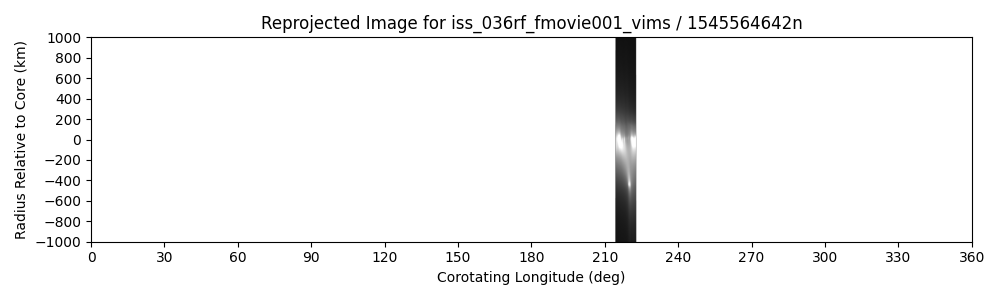
\includegraphics[width=\linewidth]{figures/screenshot-display-reproj-img.png}

\begin{CodeBlock}
$ python plot_ews_ma.py \
    /path/to/bundle/data_mosaic_bkg_sub/iss_036rf_fmovie001_vims/iss_036rf_fmovie001_vims_mosaic_bkg_sub.lblx
\end{CodeBlock}

\noindent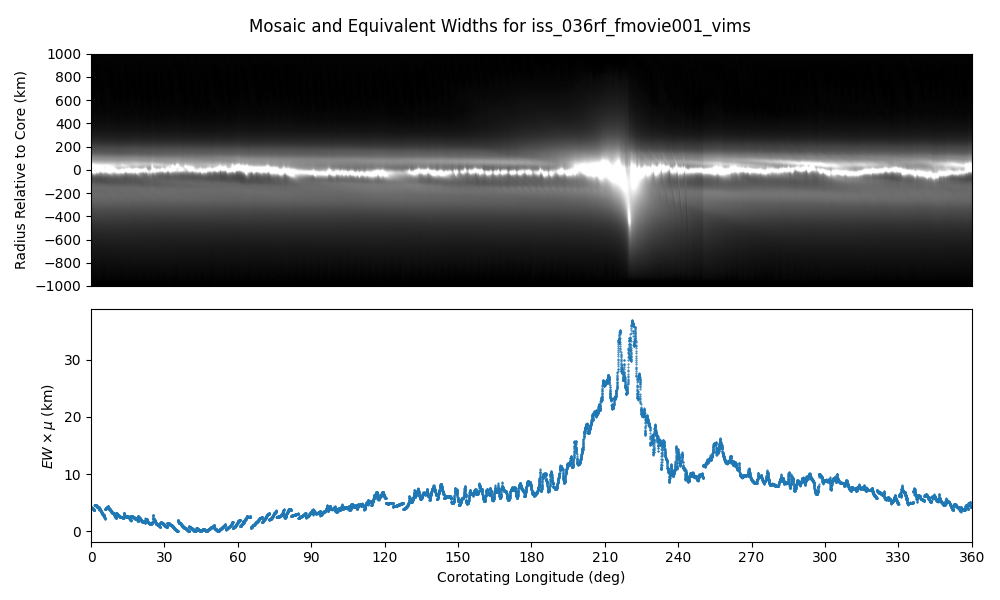
\includegraphics[width=\linewidth]{figures/screenshot-plot-ews.png}

\begin{CodeBlock}
$ python find_prometheus_closest_approaches.py /path/to/bundle
\end{CodeBlock}

\noindent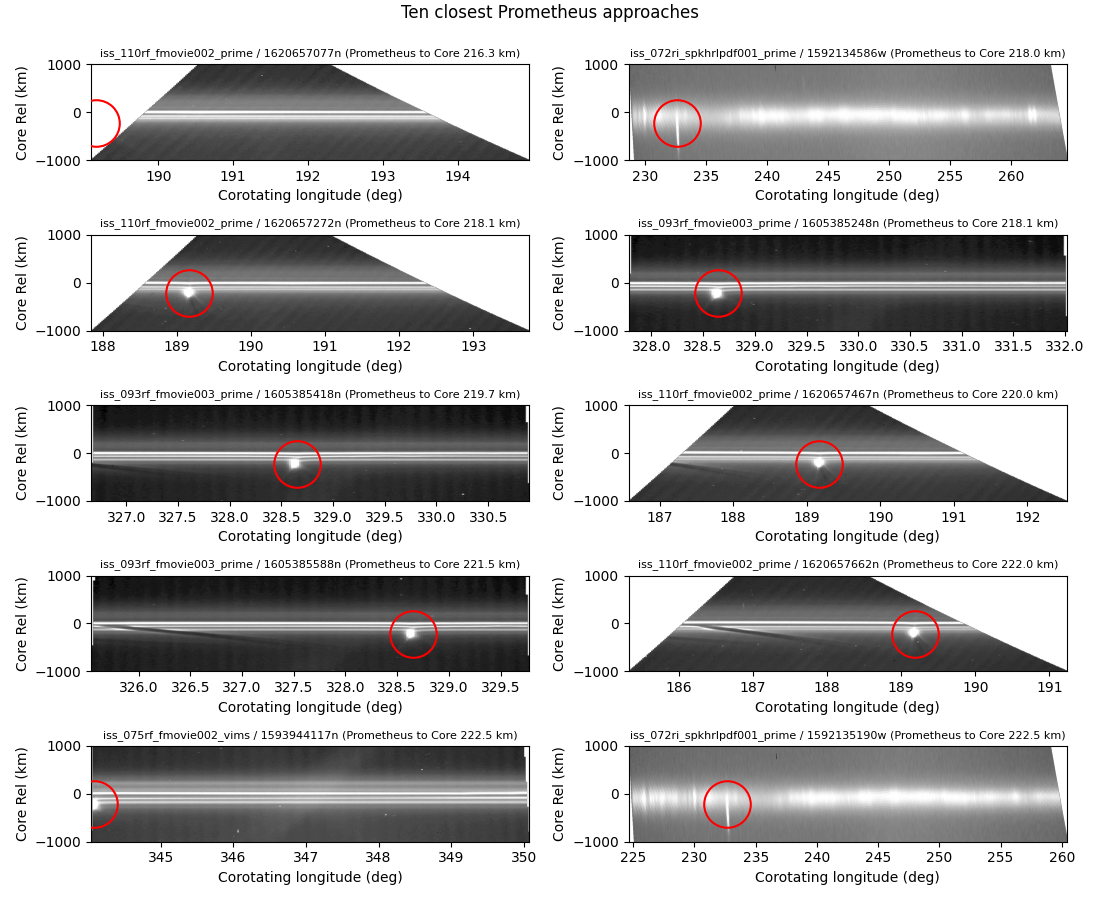
\includegraphics[width=\linewidth]{figures/screenshot-find-prometheus.png}


\subsubsection{F ring bundle analysis programs}
\label{sec:f-ring-bundle-analysis-programs}

In addition to the example programs included with the archived bundle, additional software is available to aid researchers in viewing and analyzing the data. As this software evolves rapidly, it is not included with the bundle, but is instead available in this GitHub repo:

\href{https://github.com/SETI/fring-mosaics-bundle-software}{https://github.com/SETI/fring-mosaics-bundle-software}

\clearpage
% Section 6: External references and further reading

\section{External references and further reading}
\label{sec:external-references-and-further-reading}

This section provides a curated list of external references, documentation, and further reading relevant to the Saturn F Ring Cassini ISS Mosaic Bundle.


\subsection{PDS4 standards and documentation}
\label{sec:pds4-standards-and-documentation}

\begin{itemize}
\item NASA Planetary Data System (PDS) Home: \url{https://pds.nasa.gov/}
\item PDS4 Documents: \url{https://pds.nasa.gov/datastandards/documents/}
\item PDS4 Information Model Specification: \url{https://pds.nasa.gov/datastandards/documents/im/}
\item PDS4 Data Dictionaries: \url{https://pds.nasa.gov/datastandards/dictionaries/}
\end{itemize}

\subsection{Cassini mission and instrumentation}
\label{sec:cassini-mission-and-instrumentation}

\begin{itemize}
\item Cassini-Huygens Mission Overview: \url{https://saturn.jpl.nasa.gov/mission/}
\item Cassini ISS (Imaging Science Subsystem) Overview: \url{https://pds-atmospheres.nmsu.edu/data_and_services/atmospheres_data/Cassini/inst-iss.html}
\item Cassini ISS Data User Guide (PDS3): \url{https://doi.org/10.17189/1504135}
\item Cassini ISS Narrow Angle Camera (NAC) Details: \url{https://pds-rings.seti.org/pds4/bundles/cassini_iss_saturn/document/iss-na-camera-description.txt}
\item Cassini ISS Wide Angle Camera (WAC) Details: \url{https://pds-rings.seti.org/pds4/bundles/cassini_iss_saturn/document/iss-wa-camera-description.txt}
\end{itemize}

\subsection{SPICE toolkit}
\label{sec:spice-toolkit}

\begin{itemize}
\item SPICE Toolkit Documentation: \url{https://naif.jpl.nasa.gov/naif/documentation.html}
\item SPICE Tutorials and Reference: \url{https://naif.jpl.nasa.gov/naif/tutorials.html}
\end{itemize}

\subsection{Additional resources}
\label{sec:additional-resources}

\begin{itemize}
\item PDS Ring-Moon Systems Node: \url{https://pds-rings.seti.org/}
\item PDS Small Bodies Node: \href{https://pdssbn.astro.umd.edu/}{https://pdssbn.astro.umd.edu/}
\item PDS Cartography and Imaging Sciences Node: \url{https://pds-imaging.jpl.nasa.gov/}
\clearpage
\end{itemize}

\subsection{References}
\label{sec:references}

\noindent\hangindent=2em\hangafter=1 Albers, N., Sremčević, M., Colwell, J. E., \& Esposito, L. W. 2012, Icarus, 217, 367

\noindent\hangindent=2em\hangafter=1 Attree, N., Murray, C., Cooper, N. J., \& Williams, G. 2012, AGU Fall Meet Abstr, 54, P54B

\noindent\hangindent=2em\hangafter=1 Attree, N. O., Murray, C. D., Williams, G. A., \& Cooper, N. J. 2014, Icarus, 227, 56

\noindent\hangindent=2em\hangafter=1 Beurle, K., Murray, C. D., Williams, G. A., et al. 2010, Astrophys J, 718, L176

\noindent\hangindent=2em\hangafter=1 Cooper, N. J., Murray, C. D., \& Williams, G. A. 2013, Astron J, 145, 161

\noindent\hangindent=2em\hangafter=1 Cuzzi, J. N., Marouf, E. A., French, R. G., Murray, C. D., \& Cooper, N. J. 2024, Sci Adv, 10 (American Association for the Advancement of Science), eadl6601

\noindent\hangindent=2em\hangafter=1 French, R. S., Hicks, S. K., Showalter, M. R., Antonsen, A. K., \& Packard, D. R. 2014a, Icarus, 241, 200

\noindent\hangindent=2em\hangafter=1 French, R. S., Showalter, M. R., \& Gordon, M. K. 2014b, AASDivision Planet Sci Meet Abstr 46, 46, \url{http://adsabs.harvard.edu/abs/2014DPS....4642201F}

\noindent\hangindent=2em\hangafter=1 French, R. S., Showalter, M. R., \& Gordon, M. K. 2016, AASDivision Planet Sci Meet Abstr 48, 121.14

\noindent\hangindent=2em\hangafter=1 French, R. S., Showalter, M. R., Sfair, R., et al. 2012, Icarus, 219, 181

\noindent\hangindent=2em\hangafter=1 Gehrels, T., Baker, L. R., Beshore, E., et al. 1980, Science, 207, 434

\noindent\hangindent=2em\hangafter=1 Knowles, B. 2018, Cassini Imaging Science Subsystem (ISS) Data User’s Guide, \url{https://pds.nasa.gov/data/pds4/releases/rings/cassini_docs-20210211/iss-data-user-guide.pdf}

\noindent\hangindent=2em\hangafter=1 Murray, C. D., Beurle, K., Cooper, N. J., et al. 2008, Nature, 453, 739

\noindent\hangindent=2em\hangafter=1 Murray, C. D., Chavez, C., Beurle, K., et al. 2005, Nature, 437, 1326

\noindent\hangindent=2em\hangafter=1 Porco, C. C., West, R. A., Squyres, S., et al. 2004, Space Sci Rev, 115, 363

\clearpage

% Section 7 is a landscape section in the Word original (its three metadata
% tables are wider than a portrait page).
\begin{rotatedlandscape}
% Section 7: Metadata and global index file fields

\section{Metadata and global index file fields}
\label{sec:metadata-and-global-index-file-fields}


\subsection{Reprojected image and mosaic metadata params}
\label{sec:reprojected-image-and-mosaic-metadata-params}

Units are uniform throughout this section and throughout the bundle. All angles, longitudes, and true anomalies are in degrees; all radii and radial distances are in km; radial resolution is in km/pixel and longitudinal resolution in degrees/pixel; coverage is given in percent; and all times given as \code{tdb} (including \code{rings:\allowbreak{}observed\_\allowbreak{}event\_\allowbreak{}tdb}) are ephemeris times in seconds past the J2000 epoch, 2000-01-01T12:00:00 Barycentric Dynamical Time (TDB) — the same quantity SPICE calls \textit{ET}. Times given as \code{date\_\allowbreak{}time} are Coordinated Universal Time (UTC).

The following fields are tabulated for each valid corotating longitude in each reprojected image (\code{IMGID\_\allowbreak{}reproj\_\allowbreak{}img\_\allowbreak{}metadata\_\allowbreak{}params.\allowbreak{}tab}), mosaic (\code{OBSID\_\allowbreak{}mosaic\_\allowbreak{}metadata\_\allowbreak{}params.\allowbreak{}tab}), and background-subtracted mosaic (\code{OBSID\_\allowbreak{}mosaic\_\allowbreak{}bkg\_\allowbreak{}sub\_\allowbreak{}metadata\_\allowbreak{}params.\allowbreak{}tab}).

\begingroup\small
\begin{longtable}{|>{\raggedright\arraybackslash}p{0.255\linewidth}|>{\raggedright\arraybackslash}p{0.665\linewidth}|}
\hline
\code{rings:\allowbreak{}corotating\_\allowbreak{}ring\_\allowbreak{}longitude} & The corotating longitude for which values are being provided \\
\hline
\code{image\_\allowbreak{}index} & (Mosaics only) The number of the reprojected image (from \code{OBSID\_\allowbreak{}mosaic\_\allowbreak{}metadata\_\allowbreak{}src\_\allowbreak{}imgs.\allowbreak{}tab} or \code{OBSID\_\allowbreak{}mosaic\_\allowbreak{}bkg\_\allowbreak{}sub\_\allowbreak{}metadata\_\allowbreak{}src\_\allowbreak{}imgs.\allowbreak{}tab}) that provided data for this corotating longitude \\
\hline
\code{rings:\allowbreak{}observed\_\allowbreak{}event\_\allowbreak{}tdb} & The mid-time of the observation that provided data for this corotating longitude (constant for one image) \\
\hline
\code{rings:\allowbreak{}inertial\_\allowbreak{}ring\_\allowbreak{}longitude} & The inertial longitude of the part of the source image that provided data for this corotating longitude \\
\hline
\code{rings:\allowbreak{}radial\_\allowbreak{}resolution} & The radial resolution of the part of the source image that provided data for this corotating longitude \\
\hline
\code{rings:\allowbreak{}longitudinal\_\allowbreak{}resolution} & The angular longitudinal resolution of the part of the source image that provided data for this corotating longitude \\
\hline
\code{rings:\allowbreak{}incidence\_\allowbreak{}angle} & The incidence angle of the ring plane at the time of the source observation (constant for one image) \\
\hline
\code{rings:\allowbreak{}phase\_\allowbreak{}angle} & The phase angle of the part of the source image that provided data for this corotating longitude \\
\hline
\code{rings:\allowbreak{}emission\_\allowbreak{}angle} & The emission angle of the part of the source image that provided data for this corotating longitude \\
\hline
\code{core\_\allowbreak{}radius} & The radius of the ideal F ring core from the orbit model at this corotating longitude \\
\hline
\code{longitude\_\allowbreak{}ascending\_\allowbreak{}node} & The longitude of the ascending node (relative to J2000) from the orbit model at the time of the source observation (constant for one image) \\
\hline
\code{longitude\_\allowbreak{}pericenter} & The longitude of pericenter (relative to J2000) from the orbit model at the time of the source observation (constant for one image) \\
\hline
\code{true\_\allowbreak{}anomaly} & The true anomaly from the orbit model corresponding to this corotating longitude \\
\hline
\code{corotating\_\allowbreak{}longitude\_\allowbreak{}prometheus} & The corotating longitude of Prometheus at the time of the source image, in the same reference frame used for the F ring core (constant for one image) \\
\hline
\code{radius\_\allowbreak{}prometheus} & The orbital radius (distance from Saturn center) of Prometheus at the time of the original observation \\
\hline
\code{corotating\_\allowbreak{}longitude\_\allowbreak{}pandora} & The corotating longitude of Pandora at the time of the source image, in the same reference frame used for the F ring core (constant for one image) \\
\hline
\code{radius\_\allowbreak{}pandora} & The orbital radius (distance from Saturn center) of Pandora at the time of the original observation \\
\hline
\end{longtable}
\endgroup


\subsection{Reprojected image global index}
\label{sec:reprojected-image-global-index}

The following fields appear in \code{global\_\allowbreak{}reproj\_\allowbreak{}img\_\allowbreak{}index.\allowbreak{}tab}.

\begingroup\small
\begin{longtable}{|>{\raggedright\arraybackslash}p{0.313\linewidth}|>{\raggedright\arraybackslash}p{0.607\linewidth}|}
\hline
\code{pds:\allowbreak{}logical\_\allowbreak{}identifier} & The PDS4 logical identifier, \textit{e.g.} \code{urn:\allowbreak{}nasa:\allowbreak{}pds:\allowbreak{}cassini\_\allowbreak{}iss\_\allowbreak{}fring\_\allowbreak{}mosaics\_\allowbreak{}rsfrench2025:\allowbreak{}}\newline \code{data\_\allowbreak{}reproj\_\allowbreak{}img:\allowbreak{}1874525875w\_\allowbreak{}reproj\_\allowbreak{}img} \\
\hline
\code{cassini:\allowbreak{}observation\_\allowbreak{}id} & The Cassini observation name of the source image, \textit{e.g.} \code{IOSIC\_\allowbreak{}276RB\_\allowbreak{}COMPLITB3001\_\allowbreak{}SI} \\
\hline
\code{file\_\allowbreak{}spec} & The path to the reprojected image label file relative to the bundle root, \textit{e.g.} \code{data\_\allowbreak{}reproj\_\allowbreak{}img/\allowbreak{}iosic\_\allowbreak{}276rb\_\allowbreak{}complitb3001\_\allowbreak{}si/\allowbreak{}}\newline \code{1874525875w\_\allowbreak{}reproj\_\allowbreak{}img.\allowbreak{}lblx} \\
\hline
\code{pds:\allowbreak{}start\_\allowbreak{}date\_\allowbreak{}time} & The start time of the source image exposure, \textit{e.g.} \code{2017-05-26T20:\allowbreak{}29:\allowbreak{}10Z} \\
\hline
\code{pds:\allowbreak{}stop\_\allowbreak{}date\_\allowbreak{}time} & The stop time of the source image exposure \\
\hline
\code{cassini:\allowbreak{}spacecraft\_\allowbreak{}clock\_\allowbreak{}start\_\allowbreak{}count} & The starting spacecraft clock count of the source image without the partition number (which is always \code{1/\allowbreak{}}) \\
\hline
\code{cassini:\allowbreak{}spacecraft\_\allowbreak{}clock\_\allowbreak{}stop\_\allowbreak{}count} & The ending spacecraft clock count of the source image without the partition number (which is always \code{1/\allowbreak{}}) \\
\hline
\code{num\_\allowbreak{}valid\_\allowbreak{}longitudes} & The number of discrete longitudes (radial slices) that contain valid data; each radial slice represents 0.02° of corotating longitude \\
\hline
\code{percent\_\allowbreak{}coverage} & The percentage of 360° containing valid data; computed as \code{num\_\allowbreak{}valid\_\allowbreak{}longitudes} / 18,000 × 100 \\
\hline
\code{rings:\allowbreak{}minimum\_\allowbreak{}corotating\_\allowbreak{}ring\_\allowbreak{}longitude} & The minimum corotating longitude, representing the left edge of the reprojected image \\
\hline
\code{rings:\allowbreak{}maximum\_\allowbreak{}corotating\_\allowbreak{}ring\_\allowbreak{}longitude} & The maximum corotating longitude, representing the right edge of the reprojected image; note that it is possible for min > max, in which case the corotating range wraps around at 360° \\
\hline
\code{rings:\allowbreak{}minimum\_\allowbreak{}inertial\_\allowbreak{}ring\_\allowbreak{}longitude} & The minimum inertial longitude from the source image used to create the reprojected image \\
\hline
\code{rings:\allowbreak{}maximum\_\allowbreak{}inertial\_\allowbreak{}ring\_\allowbreak{}longitude} & The maximum inertial longitude from the source image used to create the reprojected image; because this is a single exposure, the corotating and inertial longitude ranges have the same width \\
\hline
\code{rings:\allowbreak{}mean\_\allowbreak{}phase\_\allowbreak{}angle} & The mean (across all valid longitudes) phase angle \\
\hline
\code{rings:\allowbreak{}minimum\_\allowbreak{}phase\_\allowbreak{}angle} & The minimum (across all valid longitudes) phase angle \\
\hline
\code{rings:\allowbreak{}maximum\_\allowbreak{}phase\_\allowbreak{}angle} & The maximum (across all valid longitudes) phase angle \\
\hline
\code{rings:\allowbreak{}mean\_\allowbreak{}incidence\_\allowbreak{}angle} & The ring plane incidence angle at the time of the observation. The incidence angle does not vary with longitude and changes only slowly with time, so a single value is computed for the whole product; \code{rings:\allowbreak{}minimum\_\allowbreak{}incidence\_\allowbreak{}angle} and \code{rings:\allowbreak{}maximum\_\allowbreak{}incidence\_\allowbreak{}angle} are present in the label and carry that same value \\
\hline
\code{rings:\allowbreak{}mean\_\allowbreak{}emission\_\allowbreak{}angle} & The mean (across all valid longitudes) emission angle; the angle is < 90° on the lit side of the rings \\
\hline
\code{rings:\allowbreak{}minimum\_\allowbreak{}emission\_\allowbreak{}angle} & The minimum (across all valid longitudes) emission angle \\
\hline
\code{rings:\allowbreak{}maximum\_\allowbreak{}emission\_\allowbreak{}angle} & The maximum (across all valid longitudes) emission angle \\
\hline
\code{rings:\allowbreak{}mean\_\allowbreak{}radial\_\allowbreak{}resolution} & The mean (across all valid longitudes) radial resolution in km/pixel; radial resolution is the resolution in the radial direction of the source image used to populate each reprojected image pixel \\
\hline
\code{rings:\allowbreak{}minimum\_\allowbreak{}radial\_\allowbreak{}resolution} & The minimum (across all valid longitudes) radial resolution in km/pixel \\
\hline
\code{rings:\allowbreak{}maximum\_\allowbreak{}radial\_\allowbreak{}resolution} & The maximum (across all valid longitudes) radial resolution in km/pixel \\
\hline
\code{rings:\allowbreak{}mean\_\allowbreak{}longitudinal\_\allowbreak{}resolution} & The mean (across all valid longitudes) angular longitudinal resolution in °/pixel; angular longitudinal resolution is the resolution in the longitude direction (expressed as an angle) of the source image used to populate each reprojected image pixel \\
\hline
\code{rings:\allowbreak{}minimum\_\allowbreak{}longitudinal\_\allowbreak{}resolution} & The minimum (across all valid longitudes) angular longitudinal resolution in °/pixel \\
\hline
\code{rings:\allowbreak{}maximum\_\allowbreak{}longitudinal\_\allowbreak{}resolution} & The maximum (across all valid longitudes) angular longitudinal resolution in °/pixel \\
\hline
\code{rings:\allowbreak{}minimum\_\allowbreak{}ring\_\allowbreak{}radius} & The minimum (across all valid longitudes) ring radius (distance from Saturn center) in the original image used to provide data at any valid longitude \\
\hline
\code{rings:\allowbreak{}maximum\_\allowbreak{}ring\_\allowbreak{}radius} & The maximum (across all valid longitudes) ring radius (distance from Saturn center) in the original image used to provide data at any valid longitude \\
\hline
\code{mean\_\allowbreak{}core\_\allowbreak{}radius} & The mean (across all valid longitudes) ring radius (distance from Saturn center) of the ideal F ring core from the orbit model (Section~\ref{sec:f-ring-orbit}) \\
\hline
\code{minimum\_\allowbreak{}core\_\allowbreak{}radius} & The minimum (across all valid longitudes) ring radius (distance from Saturn center) of the F ring core from the orbit model \\
\hline
\code{maximum\_\allowbreak{}core\_\allowbreak{}radius} & The maximum (across all valid longitudes) ring radius (distance from Saturn center) of the F ring core from the orbit model \\
\hline
\code{longitude\_\allowbreak{}ascending\_\allowbreak{}node} & The longitude of the ascending node of the F ring (relative to J2000) from the orbit model at the time of the original observation (Section~\ref{sec:f-ring-orbit}) \\
\hline
\code{longitude\_\allowbreak{}pericenter} & The longitude of pericenter of the F ring (relative to J2000) from the orbit model at the time of the original observation (Section~\ref{sec:f-ring-orbit}) \\
\hline
\code{minimum\_\allowbreak{}true\_\allowbreak{}anomaly} & The minimum (across all valid longitudes) true anomaly from the orbit model (Section~\ref{sec:f-ring-orbit}) \\
\hline
\code{maximum\_\allowbreak{}true\_\allowbreak{}anomaly} & The maximum (across all valid longitudes) true anomaly from the orbit model (Section~\ref{sec:f-ring-orbit}) \\
\hline
\code{corotating\_\allowbreak{}longitude\_\allowbreak{}prometheus} & The corotating longitude of Prometheus at the time of the original observation in the same reference frame used for the F ring core \\
\hline
\code{radius\_\allowbreak{}prometheus} & The orbital radius (distance from Saturn center) of Prometheus at the time of the original observation \\
\hline
\code{corotating\_\allowbreak{}longitude\_\allowbreak{}pandora} & The corotating longitude of Pandora at the time of the original observation in the same reference frame used for the F ring core \\
\hline
\code{radius\_\allowbreak{}pandora} & The orbital radius (distance from Saturn center) of Pandora at the time of the original observation \\
\hline
\code{pds:\allowbreak{}creation\_\allowbreak{}date\_\allowbreak{}time} & The date and time the reprojected image product was created \\
\hline
\code{nav\_\allowbreak{}quality} & The navigation grade of the mosaic belonging to this image’s observation. It is the overall grade for that group of images, not an assessment of this one image, and every reprojected image of the same observation carries the same value — including those that did not contribute to the mosaic (Section~\ref{sec:reprojected-images-not-used-in-a-mosaic}). Values are G = Good, F = Fair, P = Poor (Section~\ref{sec:navigation}) \\
\hline
\code{notes} & Notes about the mosaic belonging to this image’s observation (Section~\ref{sec:the-global-index-files}) \\
\hline
\end{longtable}
\endgroup


\subsection{Mosaic and background-subtracted mosaic global indexes}
\label{sec:mosaic-global-index}

The following fields appear in \code{global\_\allowbreak{}mosaic\_\allowbreak{}index.\allowbreak{}tab} and \code{global\_\allowbreak{}mosaic\_\allowbreak{}bkg\_\allowbreak{}sub\_\allowbreak{}index.\allowbreak{}tab}. Rows marked “background-subtracted mosaic only” are present only in the latter.

\begingroup\small
\begin{longtable}{|>{\raggedright\arraybackslash}p{0.313\linewidth}|>{\raggedright\arraybackslash}p{0.607\linewidth}|}
\hline
\code{pds:\allowbreak{}logical\_\allowbreak{}identifier} & The PDS4 logical identifier, \textit{e.g.} \code{urn:\allowbreak{}nasa:\allowbreak{}pds:\allowbreak{}cassini\_\allowbreak{}iss\_\allowbreak{}fring\_\allowbreak{}mosaics\_\allowbreak{}rsfrench2025:\allowbreak{}data\_\allowbreak{}mosaic:\allowbreak{}iosic\_\allowbreak{}276rb\_\allowbreak{}complitb3001\_\allowbreak{}si\_\allowbreak{}mosaic} \\
\hline
\code{cassini:\allowbreak{}observation\_\allowbreak{}id} & The Cassini observation name of the source images, \textit{e.g.} \code{IOSIC\_\allowbreak{}276RB\_\allowbreak{}COMPLITB3001\_\allowbreak{}SI} \\
\hline
\code{file\_\allowbreak{}spec} & The path to the mosaic label file relative to the bundle root, \textit{e.g.} \code{data\_\allowbreak{}mosaic/\allowbreak{}iosic\_\allowbreak{}276rb\_\allowbreak{}complitb3001\_\allowbreak{}si/\allowbreak{}iosic\_\allowbreak{}276rb\_\allowbreak{}complitb3001\_\allowbreak{}si\_\allowbreak{}mosaic.\allowbreak{}lblx} \\
\hline
\code{pds:\allowbreak{}start\_\allowbreak{}date\_\allowbreak{}time} & The start time of the earliest source image exposure, \textit{e.g.} \code{2017-05-26T20:\allowbreak{}29:\allowbreak{}10Z} \\
\hline
\code{pds:\allowbreak{}stop\_\allowbreak{}date\_\allowbreak{}time} & The stop time of the latest source image exposure \\
\hline
\code{cassini:\allowbreak{}spacecraft\_\allowbreak{}clock\_\allowbreak{}start\_\allowbreak{}count} & The starting spacecraft clock count of the earliest source image without the partition number (which is always \code{1/\allowbreak{}}) \\
\hline
\code{cassini:\allowbreak{}spacecraft\_\allowbreak{}clock\_\allowbreak{}stop\_\allowbreak{}count} & The ending spacecraft clock count of the latest source image without the partition number (which is always \code{1/\allowbreak{}}) \\
\hline
\code{num\_\allowbreak{}valid\_\allowbreak{}longitudes} & The number of discrete longitudes (radial slices) that contain valid data; each radial slice represents 0.02° of corotating longitude \\
\hline
\code{percent\_\allowbreak{}coverage} & The percentage of 360° containing valid data; computed as \code{num\_\allowbreak{}valid\_\allowbreak{}longitudes} / 18,000 × 100 \\
\hline
\code{rings:\allowbreak{}minimum\_\allowbreak{}corotating\_\allowbreak{}ring\_\allowbreak{}longitude} & The minimum corotating longitude, representing the left edge of the mosaic \\
\hline
\code{rings:\allowbreak{}maximum\_\allowbreak{}corotating\_\allowbreak{}ring\_\allowbreak{}longitude} & The maximum corotating longitude, representing the right edge of the mosaic; note that it is possible for min > max, in which case the corotating range wraps around at 360° \\
\hline
\code{rings:\allowbreak{}minimum\_\allowbreak{}inertial\_\allowbreak{}ring\_\allowbreak{}longitude} & The minimum inertial longitude from the source images used to create the mosaic \\
\hline
\code{rings:\allowbreak{}maximum\_\allowbreak{}inertial\_\allowbreak{}ring\_\allowbreak{}longitude} & The maximum inertial longitude from the source images used to create the mosaic \\
\hline
\code{rings:\allowbreak{}mean\_\allowbreak{}phase\_\allowbreak{}angle} & The mean (across all valid longitudes) phase angle \\
\hline
\code{rings:\allowbreak{}minimum\_\allowbreak{}phase\_\allowbreak{}angle} & The minimum (across all valid longitudes) phase angle \\
\hline
\code{rings:\allowbreak{}maximum\_\allowbreak{}phase\_\allowbreak{}angle} & The maximum (across all valid longitudes) phase angle \\
\hline
\code{rings:\allowbreak{}mean\_\allowbreak{}incidence\_\allowbreak{}angle} & The ring plane incidence angle during the times the source images were taken. The incidence angle does not vary with longitude and changes only slowly with time, so a single value is computed for the whole mosaic; \code{rings:\allowbreak{}minimum\_\allowbreak{}incidence\_\allowbreak{}angle} and \code{rings:\allowbreak{}maximum\_\allowbreak{}incidence\_\allowbreak{}angle} are present in the label and carry that same value \\
\hline
\code{rings:\allowbreak{}mean\_\allowbreak{}emission\_\allowbreak{}angle} & The mean (across all valid longitudes) emission angle; the angle is < 90° on the lit side of the rings \\
\hline
\code{rings:\allowbreak{}minimum\_\allowbreak{}emission\_\allowbreak{}angle} & The minimum (across all valid longitudes) emission angle \\
\hline
\code{rings:\allowbreak{}maximum\_\allowbreak{}emission\_\allowbreak{}angle} & The maximum (across all valid longitudes) emission angle \\
\hline
\code{rings:\allowbreak{}mean\_\allowbreak{}radial\_\allowbreak{}resolution} & The mean (across all valid longitudes) radial resolution in km/pixel; radial resolution is the resolution in the radial direction of the source image used to populate each mosaic pixel \\
\hline
\code{rings:\allowbreak{}minimum\_\allowbreak{}radial\_\allowbreak{}resolution} & The minimum (across all valid longitudes) radial resolution in km/pixel \\
\hline
\code{rings:\allowbreak{}maximum\_\allowbreak{}radial\_\allowbreak{}resolution} & The maximum (across all valid longitudes) radial resolution in km/pixel \\
\hline
\code{rings:\allowbreak{}mean\_\allowbreak{}longitudinal\_\allowbreak{}resolution} & The mean (across all valid longitudes) angular longitudinal resolution in °/pixel; angular longitudinal resolution is the resolution in the longitude direction (expressed as an angle) of the source image used to populate each mosaic pixel \\
\hline
\code{rings:\allowbreak{}minimum\_\allowbreak{}longitudinal\_\allowbreak{}resolution} & The minimum (across all valid longitudes) angular longitudinal resolution in °/pixel \\
\hline
\code{rings:\allowbreak{}maximum\_\allowbreak{}longitudinal\_\allowbreak{}resolution} & The maximum (across all valid longitudes) angular longitudinal resolution in °/pixel \\
\hline
\code{rings:\allowbreak{}minimum\_\allowbreak{}ring\_\allowbreak{}radius} & The minimum (across all valid longitudes) ring radius (distance from Saturn center) in the original images used to provide data at any valid longitude \\
\hline
\code{rings:\allowbreak{}maximum\_\allowbreak{}ring\_\allowbreak{}radius} & The maximum (across all valid longitudes) ring radius (distance from Saturn center) in the original images used to provide data at any valid longitude \\
\hline
\code{mean\_\allowbreak{}core\_\allowbreak{}radius} & The mean (across all valid longitudes) ring radius (distance from Saturn center) of the ideal F ring core (Section~\ref{sec:f-ring-orbit}) \\
\hline
\code{minimum\_\allowbreak{}core\_\allowbreak{}radius} & The minimum (across all valid longitudes) ring radius (distance from Saturn center) of the F ring core \\
\hline
\code{maximum\_\allowbreak{}core\_\allowbreak{}radius} & The maximum (across all valid longitudes) ring radius (distance from Saturn center) of the F ring core \\
\hline
\code{mean\_\allowbreak{}longitude\_\allowbreak{}ascending\_\allowbreak{}node} & The mean longitude of the ascending node of the F ring (relative to J2000) from the orbit model across all of the source images (Section~\ref{sec:f-ring-orbit}) \\
\hline
\code{minimum\_\allowbreak{}longitude\_\allowbreak{}ascending\_\allowbreak{}node} & The minimum longitude of the ascending node of the F ring (relative to J2000) from the orbit model across all of the source images (Section~\ref{sec:f-ring-orbit}) \\
\hline
\code{maximum\_\allowbreak{}longitude\_\allowbreak{}ascending\_\allowbreak{}node} & The maximum longitude of the ascending node of the F ring (relative to J2000) from the orbit model across all of the source images (Section~\ref{sec:f-ring-orbit}) \\
\hline
\code{mean\_\allowbreak{}longitude\_\allowbreak{}pericenter} & The mean longitude of pericenter of the F ring (relative to J2000) from the orbit model across all of the source images (Section~\ref{sec:f-ring-orbit}) \\
\hline
\code{minimum\_\allowbreak{}longitude\_\allowbreak{}pericenter} & The minimum longitude of pericenter of the F ring (relative to J2000) from the orbit model across all of the source images (Section~\ref{sec:f-ring-orbit}) \\
\hline
\code{maximum\_\allowbreak{}longitude\_\allowbreak{}pericenter} & The maximum longitude of pericenter of the F ring (relative to J2000) from the orbit model across all of the source images (Section~\ref{sec:f-ring-orbit}) \\
\hline
\code{minimum\_\allowbreak{}true\_\allowbreak{}anomaly} & The minimum (across all valid longitudes) true anomaly from the orbit model (Section~\ref{sec:f-ring-orbit}) \\
\hline
\code{maximum\_\allowbreak{}true\_\allowbreak{}anomaly} & The maximum (across all valid longitudes) true anomaly from the orbit model (Section~\ref{sec:f-ring-orbit}) \\
\hline
\code{mean\_\allowbreak{}corotating\_\allowbreak{}longitude\_\allowbreak{}prometheus} & The mean corotating longitude of Prometheus in the same reference frame used for the F ring core across all source images \\
\hline
\code{minimum\_\allowbreak{}corotating\_\allowbreak{}longitude\_\allowbreak{}prometheus} & The minimum corotating longitude of Prometheus in the same reference frame used for the F ring core across all source images \\
\hline
\code{maximum\_\allowbreak{}corotating\_\allowbreak{}longitude\_\allowbreak{}prometheus} & The maximum corotating longitude of Prometheus in the same reference frame used for the F ring core across all source images \\
\hline
\code{mean\_\allowbreak{}radius\_\allowbreak{}prometheus} & The mean orbital radius (distance from Saturn center) of Prometheus across all source images \\
\hline
\code{minimum\_\allowbreak{}radius\_\allowbreak{}prometheus} & The minimum orbital radius (distance from Saturn center) of Prometheus across all source images \\
\hline
\code{maximum\_\allowbreak{}radius\_\allowbreak{}prometheus} & The maximum orbital radius (distance from Saturn center) of Prometheus across all source images \\
\hline
\code{mean\_\allowbreak{}corotating\_\allowbreak{}longitude\_\allowbreak{}pandora} & The mean corotating longitude of Pandora in the same reference frame used for the F ring core across all source images \\
\hline
\code{minimum\_\allowbreak{}corotating\_\allowbreak{}longitude\_\allowbreak{}pandora} & The minimum corotating longitude of Pandora in the same reference frame used for the F ring core across all source images \\
\hline
\code{maximum\_\allowbreak{}corotating\_\allowbreak{}longitude\_\allowbreak{}pandora} & The maximum corotating longitude of Pandora in the same reference frame used for the F ring core across all source images \\
\hline
\code{mean\_\allowbreak{}radius\_\allowbreak{}pandora} & The mean orbital radius (distance from Saturn center) of Pandora across all source images \\
\hline
\code{minimum\_\allowbreak{}radius\_\allowbreak{}pandora} & The minimum orbital radius (distance from Saturn center) of Pandora across all source images \\
\hline
\code{maximum\_\allowbreak{}radius\_\allowbreak{}pandora} & The maximum orbital radius (distance from Saturn center) of Pandora across all source images \\
\hline
\code{pds:\allowbreak{}creation\_\allowbreak{}date\_\allowbreak{}time} & The date and time the mosaic product was created \\
\hline
\code{nav\_\allowbreak{}quality} & The overall quality of the navigation across all source images; values are G = Good, F = Fair, P = Poor (Section~\ref{sec:navigation}) \\
\hline
\code{bkgnd\_\allowbreak{}quality} & (Background-subtracted mosaic only) The overall quality of the background model used for this mosaic; values are G = Good, F = Fair, P = Poor (Section~\ref{sec:background-modeling}) \\
\hline
\code{notes} & Notes about the mosaic (Section~\ref{sec:the-global-index-files}) \\
\hline
\code{num\_\allowbreak{}images} & The number of reprojected images used to create this mosaic \\
\hline
\code{min\_\allowbreak{}image\_\allowbreak{}name} & The name of the earliest source image used in this mosaic \\
\hline
\code{max\_\allowbreak{}image\_\allowbreak{}name} & The name of the latest source image used in this mosaic \\
\hline
\code{bkgnd\_\allowbreak{}lower\_\allowbreak{}limit} & (Background-subtracted mosaic only) The inner edge of the background region, as a signed $\Delta r$ in km; rows between $\Delta r$ = −1000 km and this value are used for background modeling \\
\hline
\code{bkgnd\_\allowbreak{}upper\_\allowbreak{}limit} & (Background-subtracted mosaic only) The outer edge of the background region, as a signed $\Delta r$ in km; rows between this value and $\Delta r$ = +1000 km are used for background modeling \\
\hline
\end{longtable}
\endgroup

\end{rotatedlandscape}

\end{document}
